\documentclass[11pt]{article}
% Conceptual model of the Imbanuma cyclic-irrigation model: Part I the physical model
% (Beven's perceptual -> conceptual -> procedural layers, written in the elements of
% Clark et al. 2015), Part II the agent-based model (ODD+D, Mueller et al. 2013).
% Figures: python docs/figures/validation_runs.py; python docs/figures/make_figures.py
\usepackage[left=0.85in,right=0.85in,top=0.8in,bottom=0.8in]{geometry}
\usepackage{graphicx}
\usepackage[authoryear,round]{natbib}
\usepackage[table]{xcolor}
\usepackage{amsmath,amssymb}
\usepackage{booktabs}
\usepackage{array}
\usepackage{longtable}
\usepackage{float}
\usepackage{caption}
\usepackage[hidelinks]{hyperref}
\graphicspath{{figures/}}
\captionsetup{font=small,labelfont=bf}
\newcolumntype{L}[1]{>{\raggedright\arraybackslash}p{#1}}
\setlength{\parskip}{3pt}

\title{A Coupled Physical and Agent-Based Model of the Imbanuma Cyclic Irrigation System:\\
Conceptual Model}
\author{Petru Craciun}
\date{}

\begin{document}
\maketitle

\begin{abstract}
Agricultural water management in flat alluvial plains requires balancing engineered distribution channels with complex physical hydrology, a task increasingly challenged by decentralised human decision-making and climate volatility. This document sets out the conceptual model of a coupled socio-hydrological model of the Imbanuma cyclic irrigation system in Chiba Prefecture, Japan, the behavioural and physical core of a future cognitive digital twin. It is in two parts. Part~I describes the physical model, following the perceptual--conceptual--procedural layers of \citet{Beven2012} and the elements of a process-based hydrological model set out by \citet{Clark2015}: the stores of 4,002 mapped parcels, the conservation equations that bind them, the flux equations (FAO-56 dual crop coefficient, depth-driven plow-pan percolation, Darcy exchange of perched water between neighbouring parcels, Hooghoudt drain flow), the drainage network, backwater, the pumping-station pool, and the inference of how the water left over after evapotranspiration is partitioned underground at every parcel. Part~II describes the agent-based model that acts on it, following the ODD+D protocol \citep{Mueller2013ODDD}: heterogeneous, socially learning farmers with twelve behavioural traits, and a Land Improvement District pumping-station agent that dispatches water by receding-horizon control. The model generates behaviourally grounded irrigation demand under weather and supply scenarios for a downstream water-application optimiser. We report how the coupled model compares with the measured water balance of \citet{Okura2025WaterBalance} and which behavioural traits shape the demand it generates.
\end{abstract}

\tableofcontents
\newpage

% =============================================================================
\section{Introduction}
\label{sec:intro}

The Imbanuma area is a representative case of a complex, flat agricultural water system governed by a local Land Improvement District (LID), the institutional authority responsible for Japanese irrigation asset management \citep{Kada2005LID, Shiozawa2011}. Its defining hydrological characteristic is cyclic irrigation: drainage water from paddy fields is intentionally collected, pumped, and reused as an irrigation source. This architecture substantially increases regional water reuse efficiency and suppresses the discharge of nutrient-laden agricultural drainage into surrounding public water bodies \citep{Takeda2001Cyclic, Maruyama2008}, while introducing tight, non-linear couplings between field-scale irrigation decisions and the hydrological processes that return water to the pumps. Because every withdrawal, drainage, or pumping decision alters the water available elsewhere in the loop, the system is a natural candidate for a model that represents both halves: the physical movement of water, and the decisions of the people who move it.

\citet{Okura2025WaterBalance} measured the water balance of the district's two cyclic blocks for the 2021 and 2022 irrigation seasons. Irrigation, drainage, rainfall and evapotranspiration were measured or estimated; lateral subsurface flow was obtained as the residual, and was large: between 851 and 1,438\,mm a season, part of which returned to the pumping pool and was reused. That residual is not observed underground, and the decisions of individual farmers are not observed at all. The model described here supplies both: a physical model that resolves the residual at the scale at which farmers act, and an agent-based model of the farmers and the pumping station that act on it.

A digital twin is commonly described as a virtual representation of a physical system that is connected to its real-world counterpart through data exchange and synchronisation, enabling monitoring, analysis, prediction and decision support \citep{Kritzinger2018DigitalTwin, Jones2020DigitalTwin}; a \emph{cognitive} digital twin also embeds autonomous reasoning and learning within the virtual representation \citep{Tao2019DigitalTwin, Tao2021DigitalTwin, Rasheed2020DigitalTwin}. The model described here builds the two halves such a twin requires and couples them, but it is not yet synchronised with the field: in the terminology of \citet{Kritzinger2018DigitalTwin} it is a digital model. Its immediate use is as a generator of behaviourally grounded irrigation demand, under controlled weather and supply scenarios, for a downstream water-application optimiser, which can also take over the LID's role directly.

\subsection{How this document describes the model}
\label{sec:frameworks}
Two description standards are used, one for each half.

\textbf{The physical model} is described in the three layers of \citet{Beven2012}: a \emph{perceptual} model, the modeller's understanding of how water moves in the district; a \emph{conceptual} model, the equations chosen to represent it; and a \emph{procedural} model, the code that solves them. Within the conceptual layer we follow the decomposition that \citet{Clark2015} use to make process-based hydrological models comparable: (i) the control volumes and their state variables, (ii) the conservation equations, (iii) the flux parameterisations that close them, (iv) the spatial structure and connectivity, (v) the forcing and boundary conditions, (vi) the time stepping, and (vii) the parameters, each stated with its source. Describing the stores and fluxes explicitly in this way, rather than by the name of a model, follows the flexible-modelling view that a hydrological model is a particular choice among alternative stores and constitutive functions \citep{Fenicia2011Flexible}.

\textbf{The agent-based model} is described with ODD+D \citep{Mueller2013ODDD}, the extension of the ODD protocol \citep{Grimm2020ODD} for models in which human decisions are central. Its Overview, Design concepts and Details sections are followed in order, with the decision-making, learning, sensing, prediction and heterogeneity elements that ODD+D adds.

The model was designed following the Engineering Agent-Based Social Simulation (EABSS) methodology \citep{SiebersKluegl}, from problem definition and scope through behavioural archetypes to agent templates; ODD+D is used here to document the result.

% =============================================================================
\section{Study Area and Data}
\label{sec:site}

The study area is the command area of the Hakusan-Jimbee pumping station (Okura et al.'s Shiroyama-Jimbee area) on the shore of Lake Kita-Imbanuma (Figure~\ref{fig:district}). Its cyclic blocks are the North block (260.4\,ha) and the South block (263.5\,ha); the rest of the command area is irrigated without cyclic reuse. The irrigation season runs 131 days, from 17 April to 25 August. The two monitored seasons differ sharply: 791\,mm of rain fell in 2021 and 410\,mm in 2022, against a thirty-year mean of 638\,mm.

\begin{figure}[H]
\centering
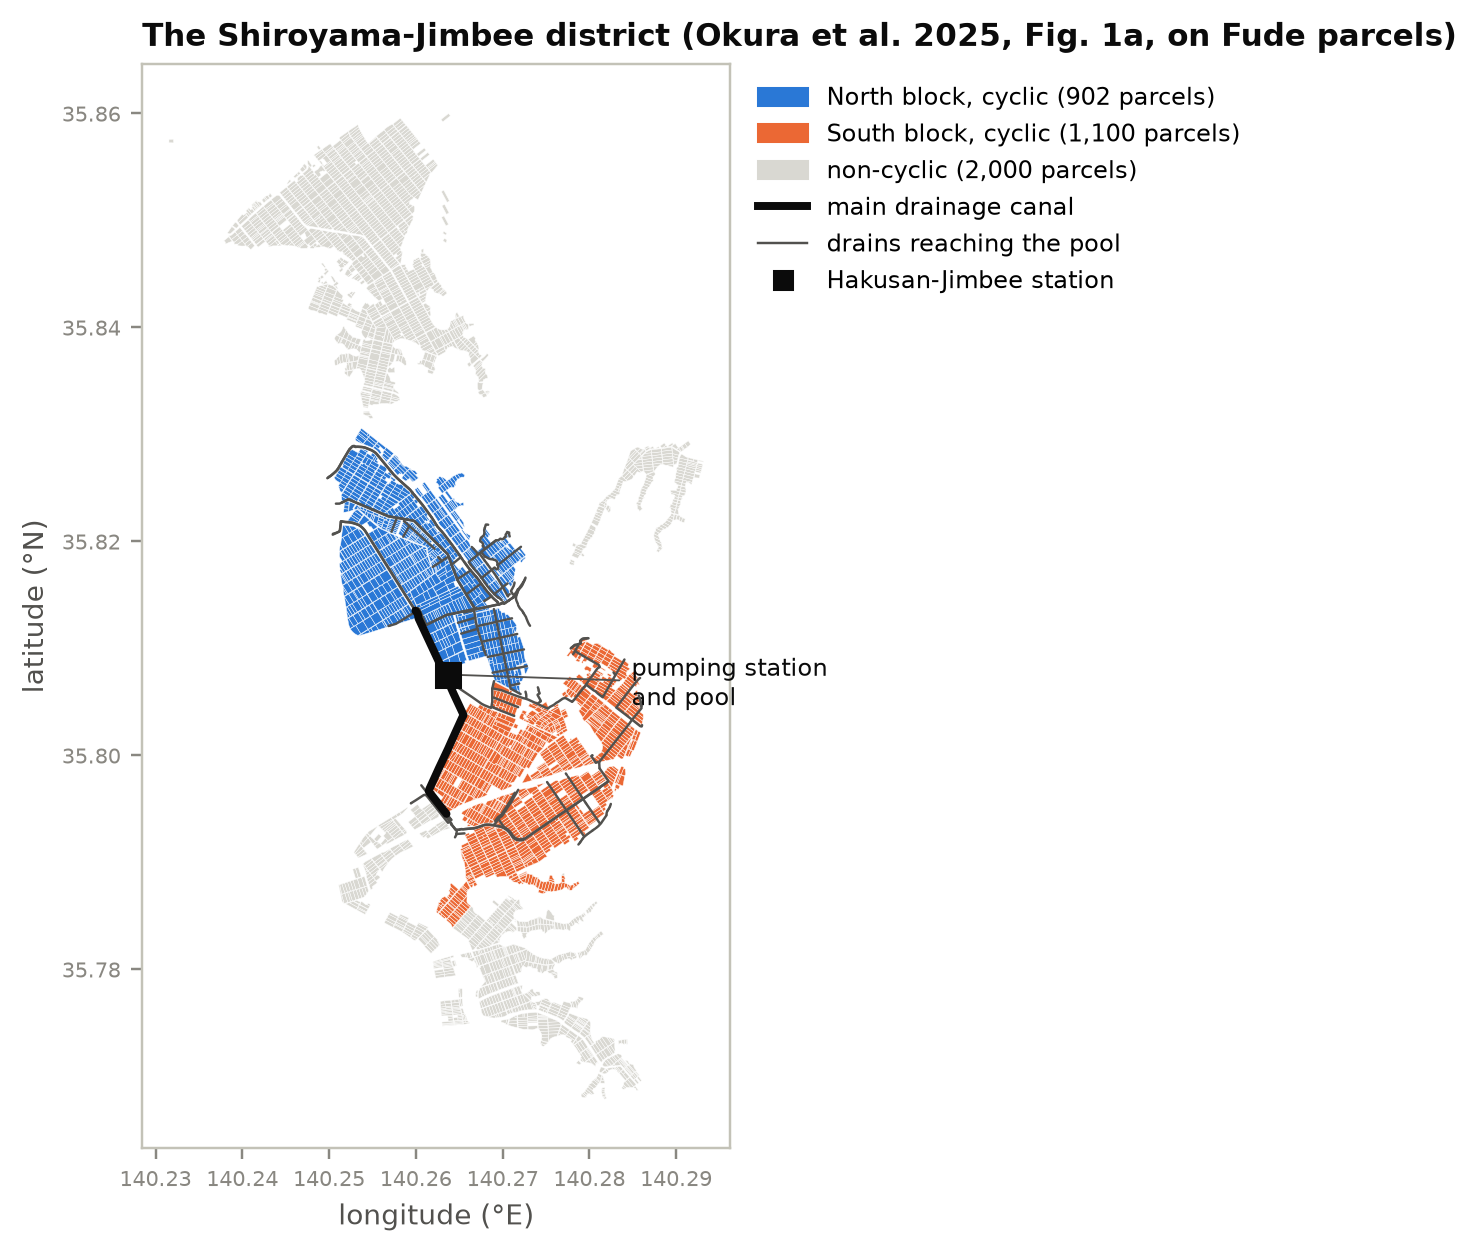
\includegraphics[width=0.92\linewidth]{fig_district}
\caption{The district as modelled: 4,002 cadastral farmland parcels (MAFF Fude polygons), classified as North cyclic, South cyclic or non-cyclic from Fig.~1a of \citet{Okura2025WaterBalance}; the drainage channels that reach the pumping-station pool (OpenStreetMap and GSI channel centrelines); the main drainage canal along the lake dyke; and the Hakusan-Jimbee pumping station.}
\label{fig:district}
\end{figure}

\begin{table}[H]
\centering\small
\begin{tabular}{L{3.6cm}L{11.6cm}}
\toprule
\textbf{Source} & \textbf{Used for} \\ \midrule
\citet{Okura2025WaterBalance} & Block water balance (Tables 2--7), main-canal depths (Fig.~3), block irrigation and drainage (Fig.~8); the pins of the recapture ratios and the validation targets. \\
MAFF Fude parcels & 4,002 parcel polygons and areas, classified from Okura Fig.~1a; areas scaled to Okura Table~1 per block. \\
OpenStreetMap, GSI & Drainage channels joined into the network that reaches the pool; main drainage canal. \\
GSI 5\,m DEM & Parcel ground elevation for the backwater rule. \\
Sentinel-2 & 10\,m NDVI, 2021 and 2022: canopy cover in the identification runs (Section~\ref{sec:identification}). \\
Open-Meteo & Daily rainfall and reference evapotranspiration ET$_0$; rainfall scaled to the on-site gauge's monthly totals (Okura Table~2). \\
MAFF Kanto & Pumping-station capacity, 3.304\,m$^3$\,s$^{-1}$; station location and layout. \\
\bottomrule
\end{tabular}
\caption{Data sources.}
\label{tab:data}
\end{table}

% =============================================================================
\part{The Physical Model}
\label{part:physical}

\section{Perceptual Model}
\label{sec:perceptual}

Water enters the district as rain on the paddies and as irrigation pumped from the pool at the Hakusan-Jimbee station through pipelines to a hydrant at each paddy (Figure~\ref{fig:perceptual}). On a paddy it stands as a shallow pond held by earth bunds and an outlet weir board. It leaves the pond in four ways: to the atmosphere by evaporation and crop transpiration; over the weir, or through the outlet when the farmer drains, into the farm drains; through the bunds and outlet structures as leakage; and downward through the compacted plow pan into the soil.

Beneath the plow pan the persistently high groundwater table of a lowland plain keeps a perched water table close to the surface, so that water which has passed the plow pan does not simply percolate away \citep{Tabuchi1985Paddy, Shiratani2004Subsurface}. It moves sideways: between neighbouring paddies, where one sits wetter than the next, a seepage path through and beneath the bunds documented in field measurements and models of paddy landscapes \citep{Huang2003Bunds, Janssen2007Fluxes, Tsubo2007Toposequence}; and towards the farm drains, which the land improvement project left dense. This lateral subsurface flow is the residual that \citet{Okura2025WaterBalance} could close only as a balance term. Part of it enters the drainage channels that reach the pool and is pumped back the same day; the rest stays in the blocks as a change in storage.

The subsurface processes the model represents are the ones the paddy literature that \citet{Okura2025WaterBalance} draw on identifies. Seepage and percolation are the main non-productive outflows of a flooded paddy, and depend on the standing water depth and the plow pan \citep{BoumanTuong2001}; infiltration in puddled, cracking paddy soils has been modelled with Darcy--Richards flow \citep{Liu2004Cracked}; return-flow models of paddy systems separate a quick surface return from a delayed subsurface one and show that a downstream field's irrigation is partly supplied by upstream return flow \citep{ChienFang2012}; water balances of rice fields in a toposequence show seepage carrying water from upslope to downslope fields \citep{Facchi2018}; and subsurface drainage of paddy fields has been modelled with both Hooghoudt's equation and the Richards equation \citep{Ebrahimian2015Hydrus}. Beyond the studies Okura et al.\ cite, lateral seepage through and beneath bunds has been measured and modelled directly \citep{Huang2003Bunds, Janssen2007Fluxes}, a Darcy-based soil-water balance underlies the SAWAH paddy model \citep{Wopereis1994SAWAH}, and lateral water movement between fields of a toposequence has been modelled as a flux between neighbouring water stores \citep{Tsubo2007Toposequence}.

Surface drainage from the cyclic blocks runs along the farm drains and the main drainage canal to the pool, taking hours over the longest routes. When the canal runs high, after heavy rain or while the station holds water back, the farm drains of the lowest parcels cannot empty into it and the water stays on the field (backwater), a behaviour \citet{Okura2025WaterBalance} identified in the North block. The pool itself is small next to a day's pumping, so it acts as a buffer: what the returns do not supply is drawn from the lake through a gate, and surplus is pumped or spills to the lake.

Two features of this picture shape everything that follows. First, the water a farmer applies does not stay on that farmer's parcel: part of it returns to the pool through drains and through the ground, and becomes the next day's irrigation elsewhere. Second, the share that returns depends on where a parcel sits relative to the drains that reach the pool.

\begin{figure}[H]
\centering
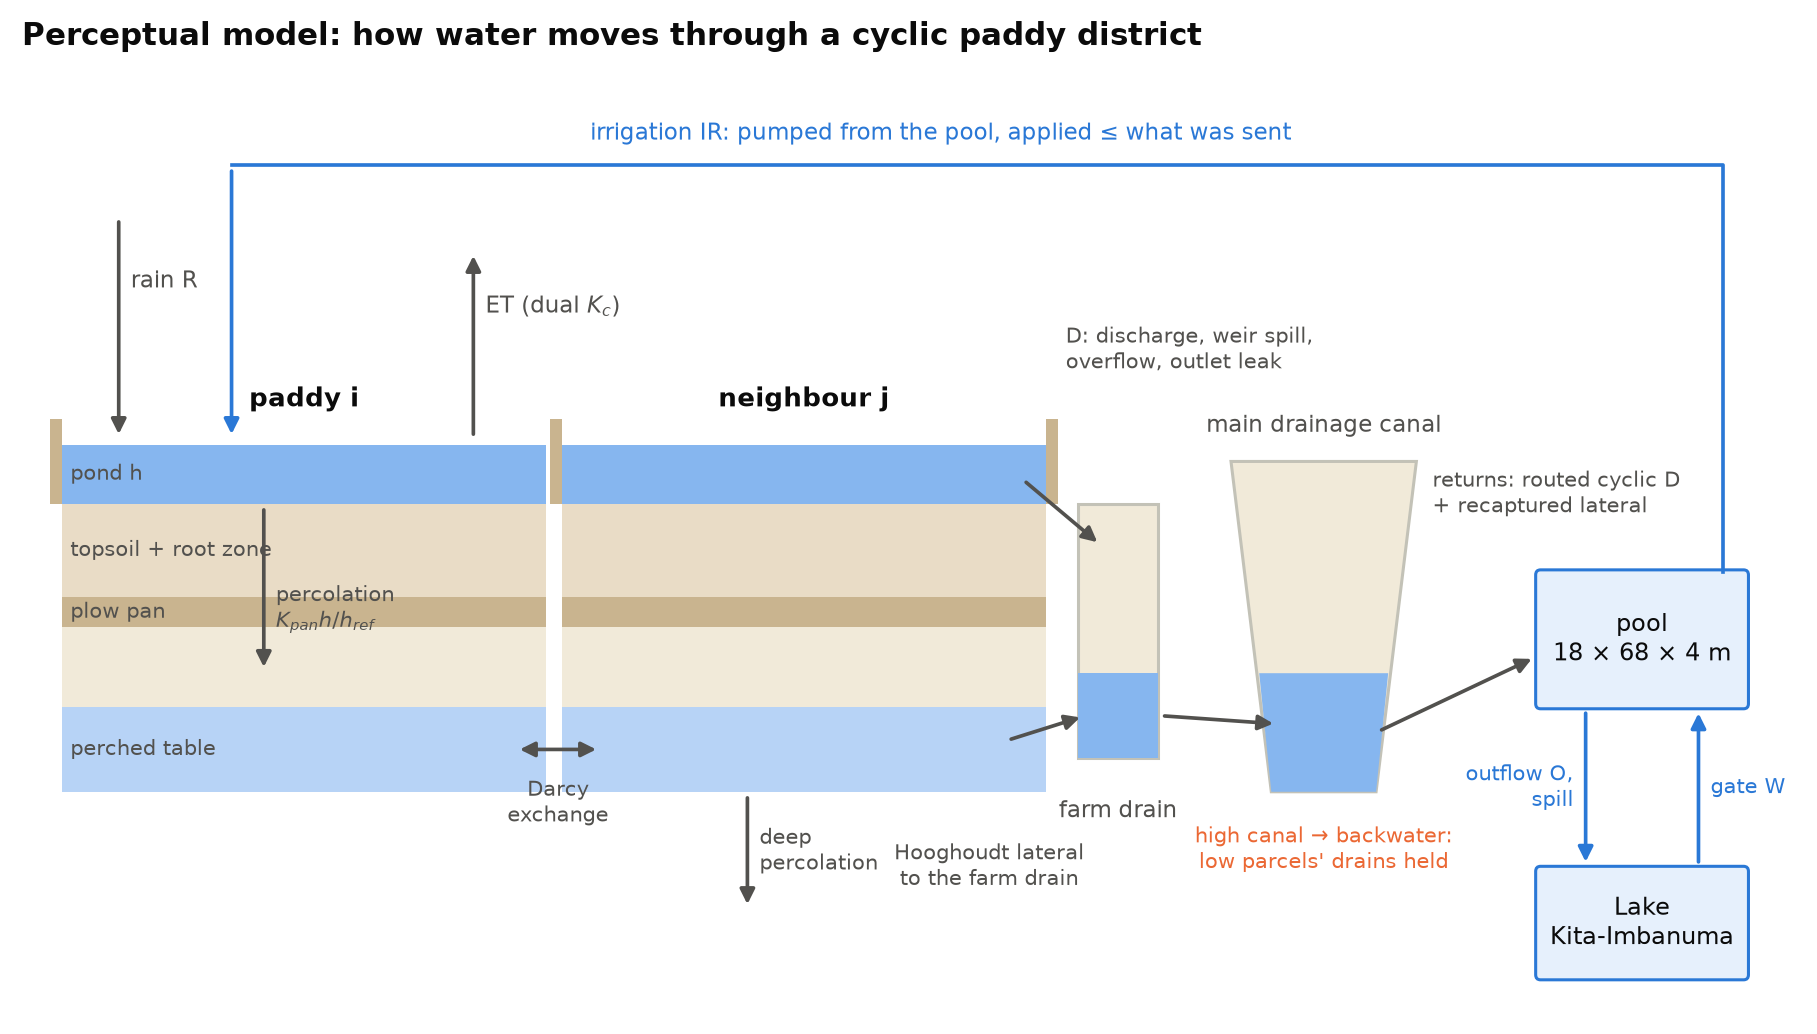
\includegraphics[width=\linewidth]{fig_perceptual}
\caption{Perceptual model: the fluxes through two neighbouring paddies, a farm drain, the main drainage canal, the pool and the lake.}
\label{fig:perceptual}
\end{figure}

% -----------------------------------------------------------------------------
\section{Conceptual Model}
\label{sec:conceptual}

Following \citet{Clark2015}, this section states the control volumes and states, the conservation equations, the flux parameterisations, the spatial structure, the forcing and boundary conditions, the time stepping and the parameters.

\subsection{Control volumes and state variables}
Each of the 4,002 parcels is a control volume with four stores, all in millimetres over the parcel's own area (Figure~\ref{fig:stores}, Table~\ref{tab:states}). The district adds the pool, the water in transit in the drains, and the block storage that \citet{Okura2025WaterBalance} denote $\Delta WB$; the lake is a boundary.

\begin{table}[H]
\centering\small
\begin{tabular}{L{3.6cm}L{1.2cm}L{10.2cm}}
\toprule
\textbf{State} & \textbf{Unit} & \textbf{Meaning} \\ \midrule
Pond $h_i$ & mm & Standing water above the soil surface. \\
Surface depletion $S_i$ & mm & Depletion of the thin evaporating layer; 0 = wet, at most TEW = 25\,mm. \\
Root-zone depletion $Z_i$ & mm & Depletion of the root zone below saturation; at most TAW = 100\,mm. \\
Perched store $P_i$ & mm & Water of the perched table above the farm-drain level. \\
Pool $V$ & m$^3$ & The $18\times68$\,m, 4\,m deep pool at the station (4,896\,m$^3$). \\
Drains in transit & m$^3$ & Cyclic surface drainage released but not yet at the pool. \\
Block storage $\Delta WB$ & m$^3$ & Lateral flow from cyclic parcels that the pool does not recapture. \\
\bottomrule
\end{tabular}
\caption{Control volumes and state variables.}
\label{tab:states}
\end{table}

\begin{figure}[H]
\centering
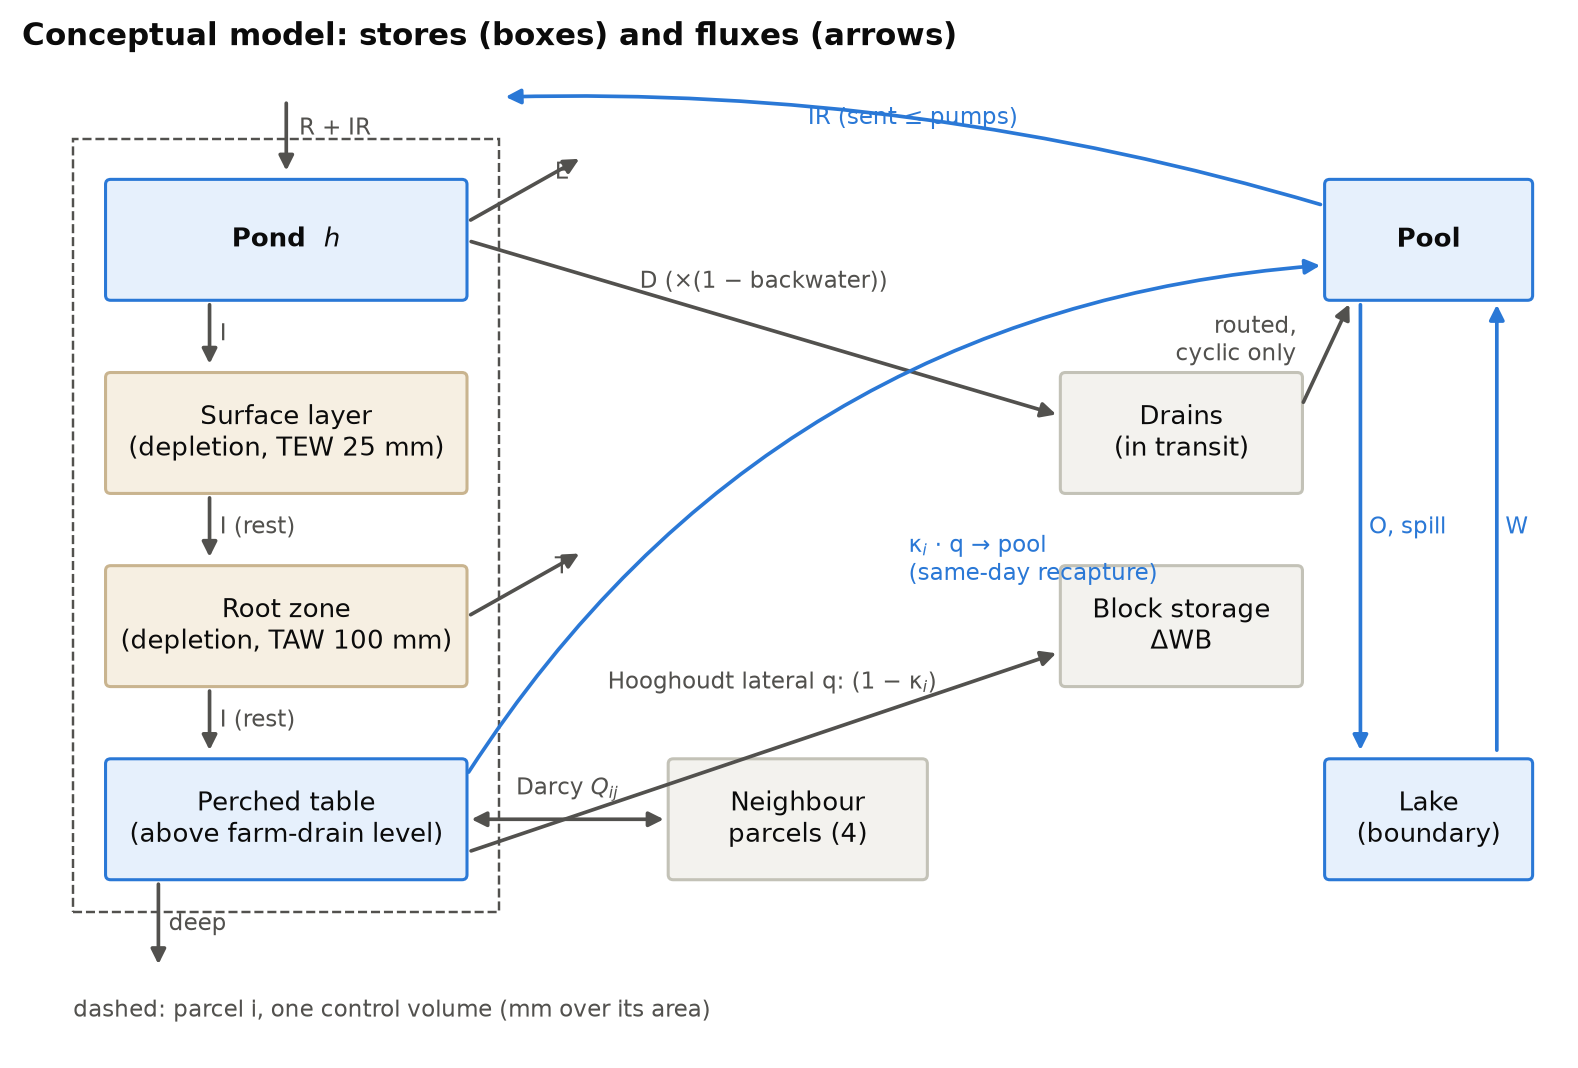
\includegraphics[width=0.92\linewidth]{fig_stores}
\caption{Conceptual model: the four stores of a parcel and the district stores they connect to. $\kappa_i$ is the parcel's recapture share (Section~\ref{sec:identification}).}
\label{fig:stores}
\end{figure}

\subsection{Conservation equations}
Every parcel conserves water each day:
\begin{equation}
\Delta\left(h_i - S_i - Z_i + P_i\right) = R + IR_i - ET_i - D_i - q_i - d_i + \sum_{j \in \mathcal{N}(i)} Q_{ji},
\label{eq:parcel}
\end{equation}
with rain $R$, applied irrigation $IR_i$, evapotranspiration $ET_i$, surface drainage $D_i$, Hooghoudt lateral flow $q_i$, deep percolation $d_i$ and the Darcy exchange $Q_{ji}$ with its neighbours $\mathcal{N}(i)$. The model checks this identity on every parcel every day.

The pool conserves water at district scale, with the identities of \citet{Okura2025WaterBalance}:
\begin{align}
\Delta V &= W - O + LFV_{pump} + D^{cyc}_{N} + D^{cyc}_{S} - IR_{all}, \label{eq:pool}\\
\Delta WB &= \tfrac{1}{1000}\big(A_N Lf_N + A_S Lf_S\big) - LFV_{pump}, \label{eq:dwb}\\
Lf_b &= IR_b + R - D_b - ET_b, \qquad b \in \{N, S\}, \label{eq:lf}
\end{align}
with lake withdrawal $W$, outflow and spill to the lake $O$, recaptured lateral flow $LFV_{pump}$, cyclic surface drainage $D^{cyc}$ arriving at the pool, total irrigation sent $IR_{all}$, block area $A_b$ and block lateral flow $Lf_b$ (their Eqs.~3, 4 and 7). The reuse ratios follow their Eqs.~12--14: $RUE = D/IR_{all}$ and $LUE = LFV_{pump}/IR_{all}$.

\subsection{Flux parameterisations}
Table~\ref{tab:fluxes} lists every flux and the equation that closes it.

\begin{table}[H]
\centering\small
\begin{tabular}{L{2.8cm}L{7.4cm}L{4.9cm}}
\toprule
\textbf{Flux} & \textbf{Parameterisation} & \textbf{Source / status} \\ \midrule
Evapo-transpiration & Dual crop coefficient, $ET = (K_s K_{cb} + K_e)ET_0$, $K_{cb} = 0.15 + (1.15 - 0.15) f_c$; $K_e$ capped at $K_{c,\max}=1.20$, or 1.29 on wetting days & \citet{Allen1998FAO56}; wetting-day cap from \citet{Xu2017DualKc} \\
Crop water stress & Demand $\min(K_{cap}, K_{cb} + f_{ew}K_{cap})\,ET_0$ met from the pond, then the surface layer; the unmet part is stress; $K_s = ET/\text{demand}$ & Model choice (rice draws on standing water and topsoil) \\
Relative yield & $Y_r = 1 - K_y\sum\text{stress}/\sum\text{demand}$, $K_y = 1.10$ & \citet{Doorenbos1979} \\
Surface drainage $D$ & Farmer's chosen discharge; pond above the weir crest; overflow above the bund; outlet leak of 13\,\% of the pond a day & Leak: assumed, to be calibrated \\
Backwater & Share of $D$ held on the parcel: $\min(1, \max(0, 1 - m_i/0.10))$, margin $m_i$ = ground elevation above the drain reference minus the canal's rise above its normal depth & \citet{Okura2025WaterBalance} Fig.~3; GSI DEM \\
Plow-pan percolation & $I = K_{pan}\,h/h_{ref}$, $K_{pan} = 9.5$\,mm\,d$^{-1}$, $h_{ref} = 30$\,mm, at most $h$ & Assumed, to be calibrated \\
Perched exchange & $Q_{ij} = K_{ij} D_{eq}(H_i - H_j)$, $H = P/(1000\mu)$, $K_{ij} = \tfrac{1}{2}[(K_{x,i}+K_{x,j})u_x^2 + (K_{y,i}+K_{y,j})u_y^2]$ & Darcy's law; bund-seepage evidence: \citet{Huang2003Bunds, Janssen2007Fluxes, Tsubo2007Toposequence} \\
Drain flow $q$ & Hooghoudt: $q = (8 K D_{eq} H + 4 K H^2)/L^2$, $K = \sqrt{K_x K_y}$ & \citet{Hooghoudt1940}; see note below \\
Deep percolation $d$ & $\min(1\,\text{mm d}^{-1}, P)$ & Assumed \\
Recapture & $\kappa_i\,q_i$ to the pool the same day on cyclic parcels; $(1-\kappa_i)q_i$ to $\Delta WB$ & Inferred (Section~\ref{sec:identification}) \\
Drain routing & Cyclic $D$ reaches the pool after route length $/\,0.2$\,m\,s$^{-1}$, spread over the arrival day & Route: mapped network; velocity assumed \\
\bottomrule
\end{tabular}
\caption{Flux parameterisations. $f_c$ is canopy cover, $f_{ew} = 1 - f_c$, $\mu = 0.15$ the drainable porosity, $D_{eq} = 0.8$\,m the equivalent depth, $L = 10$\,m the drain spacing, $K_x = K_y = 2{,}000$\,mm\,d$^{-1}$ unless calibrated.}
\label{tab:fluxes}
\end{table}

\textbf{On the choice of Hooghoudt.} Hooghoudt's equation was developed for parallel drains under ordinary fields, with radial flow near the drains and the Dupuit--Forchheimer assumptions away from them. \citet{Ebrahimian2015Hydrus}, one of the paddy-drainage studies \citet{Okura2025WaterBalance} cite, compared it with a Richards-equation model (HYDRUS-2D) of paddy fields and found that drainage rates calculated by Hooghoudt's equation were much lower, concluding that it did not perform well for paddy fields. The lateral flow simulated here is likewise well below the residual Okura et al.\ measured (Section~\ref{sec:evaluation}), which makes the drain-flow law, together with the uncalibrated conductivities, the first candidate for revision.

\subsection{Spatial structure and connectivity}
The landscape is the set of mapped parcels, not a grid. Each parcel is linked to its nearest neighbour in each of the four cardinal directions (east, west, north, south, chosen among its eight nearest parcels by dominant axis); these edges carry the Darcy exchange. Each cyclic parcel is linked to the drainage network by the length of its route to the pool: the distance to the nearest mapped channel that reaches the pool, plus the distance along the channels. The recapture share $\kappa_i$ of each parcel is a function of its distance to that network (Figure~\ref{fig:recapture}). Non-cyclic parcels drain to the lake and the Tone River and do not contribute to the pool.

\subsection{Forcing and boundary conditions}
Rainfall and ET$_0$ are daily Open-Meteo series for the district; rainfall is scaled month by month to the totals of the on-site gauge reported by \citet{Okura2025WaterBalance} (their Table~2), because the reanalysis overstates season rainfall at Imbanuma by 30--50\,\%. The main-canal depth at the North and South arms is the daily series of their Fig.~3. Lake Kita-Imbanuma is an unlimited boundary: withdrawals are never limited by it. The pumping station cannot lift more than 3.304\,m$^3$\,s$^{-1}$; when the requested send exceeds what is available, parcels nearest the pool are served first. Figure~\ref{fig:forcing} shows the forcing of the two seasons.

\begin{figure}[H]
\centering
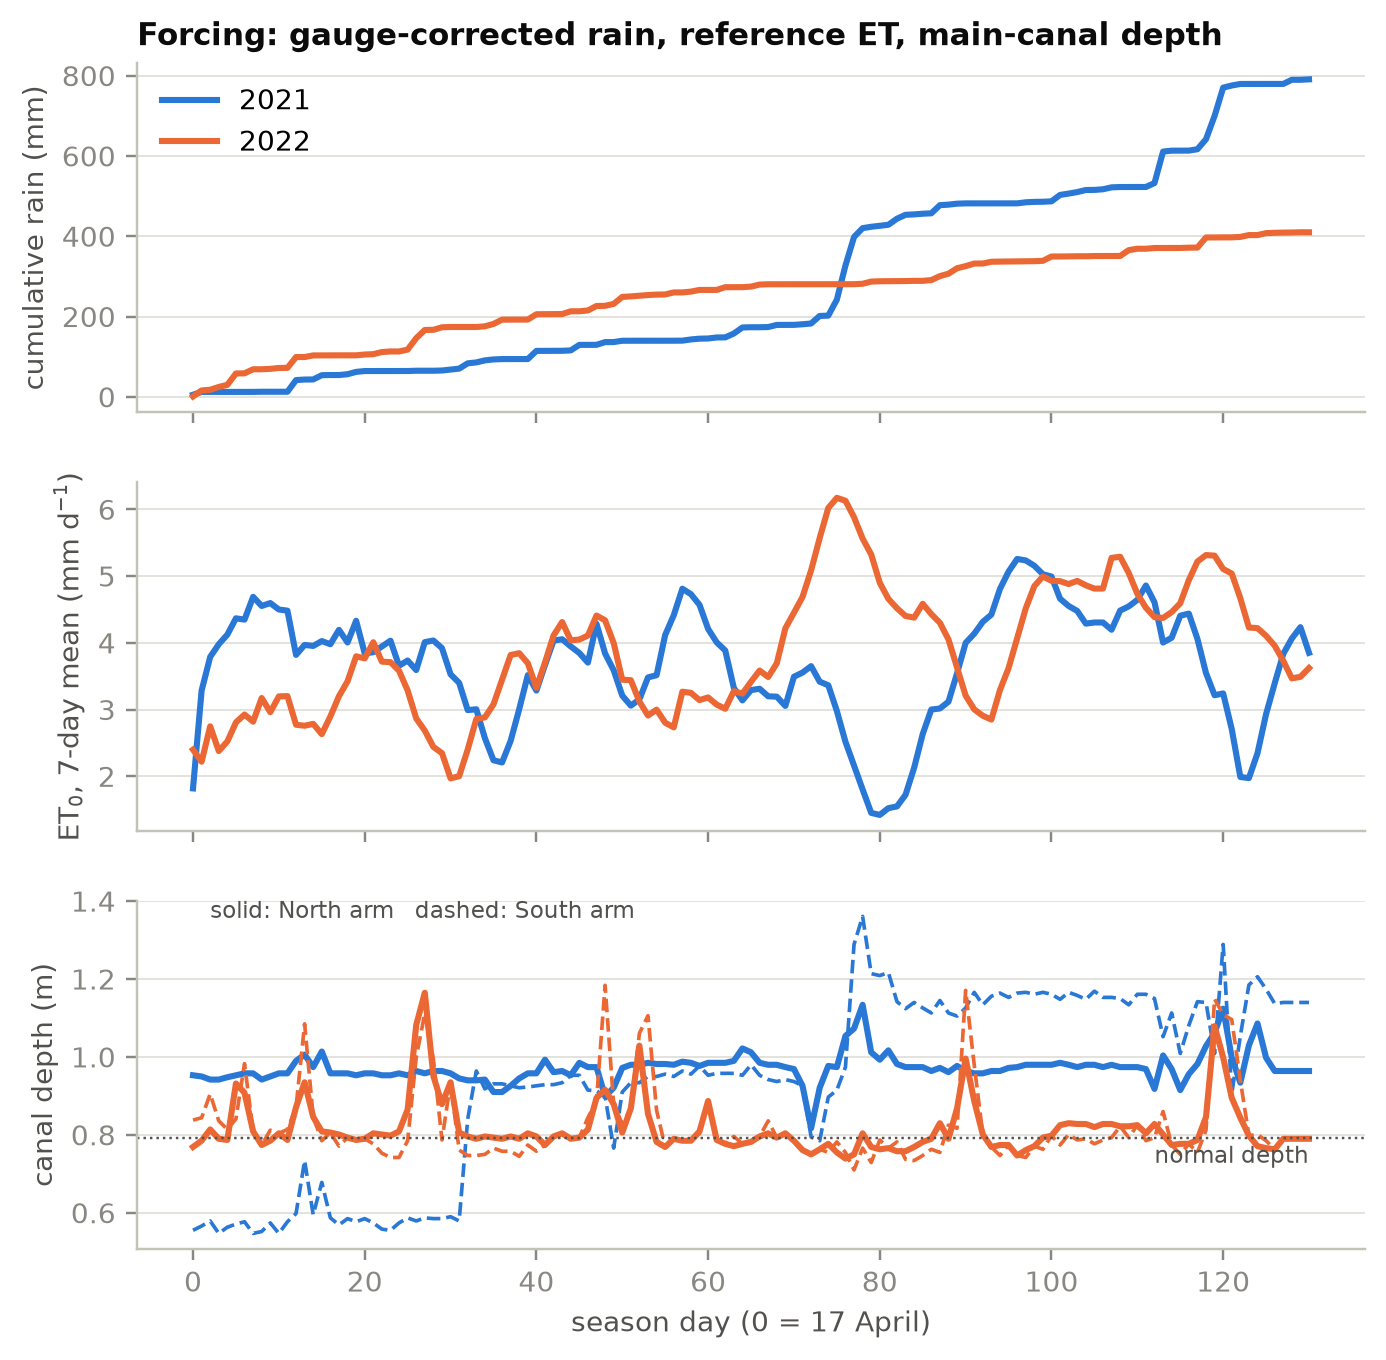
\includegraphics[width=0.82\linewidth]{fig_forcing}
\caption{Forcing for the two monitored seasons: cumulative gauge-corrected rain, 7-day mean ET$_0$, and the daily depth of the main drainage canal at its North (solid) and South (dashed) arms, from \citet{Okura2025WaterBalance} Fig.~3.}
\label{fig:forcing}
\end{figure}

\subsection{Time stepping and process order}
The model advances in daily steps, every parcel at once, in the order of Figure~\ref{fig:order}. The order matters: evapotranspiration is taken before drainage and percolation, so that a pond the farmer drains does not also evaporate; backwater is applied to the drainage after it is computed; and the pool is settled last, once the day's returns are known.

\begin{figure}[H]
\centering
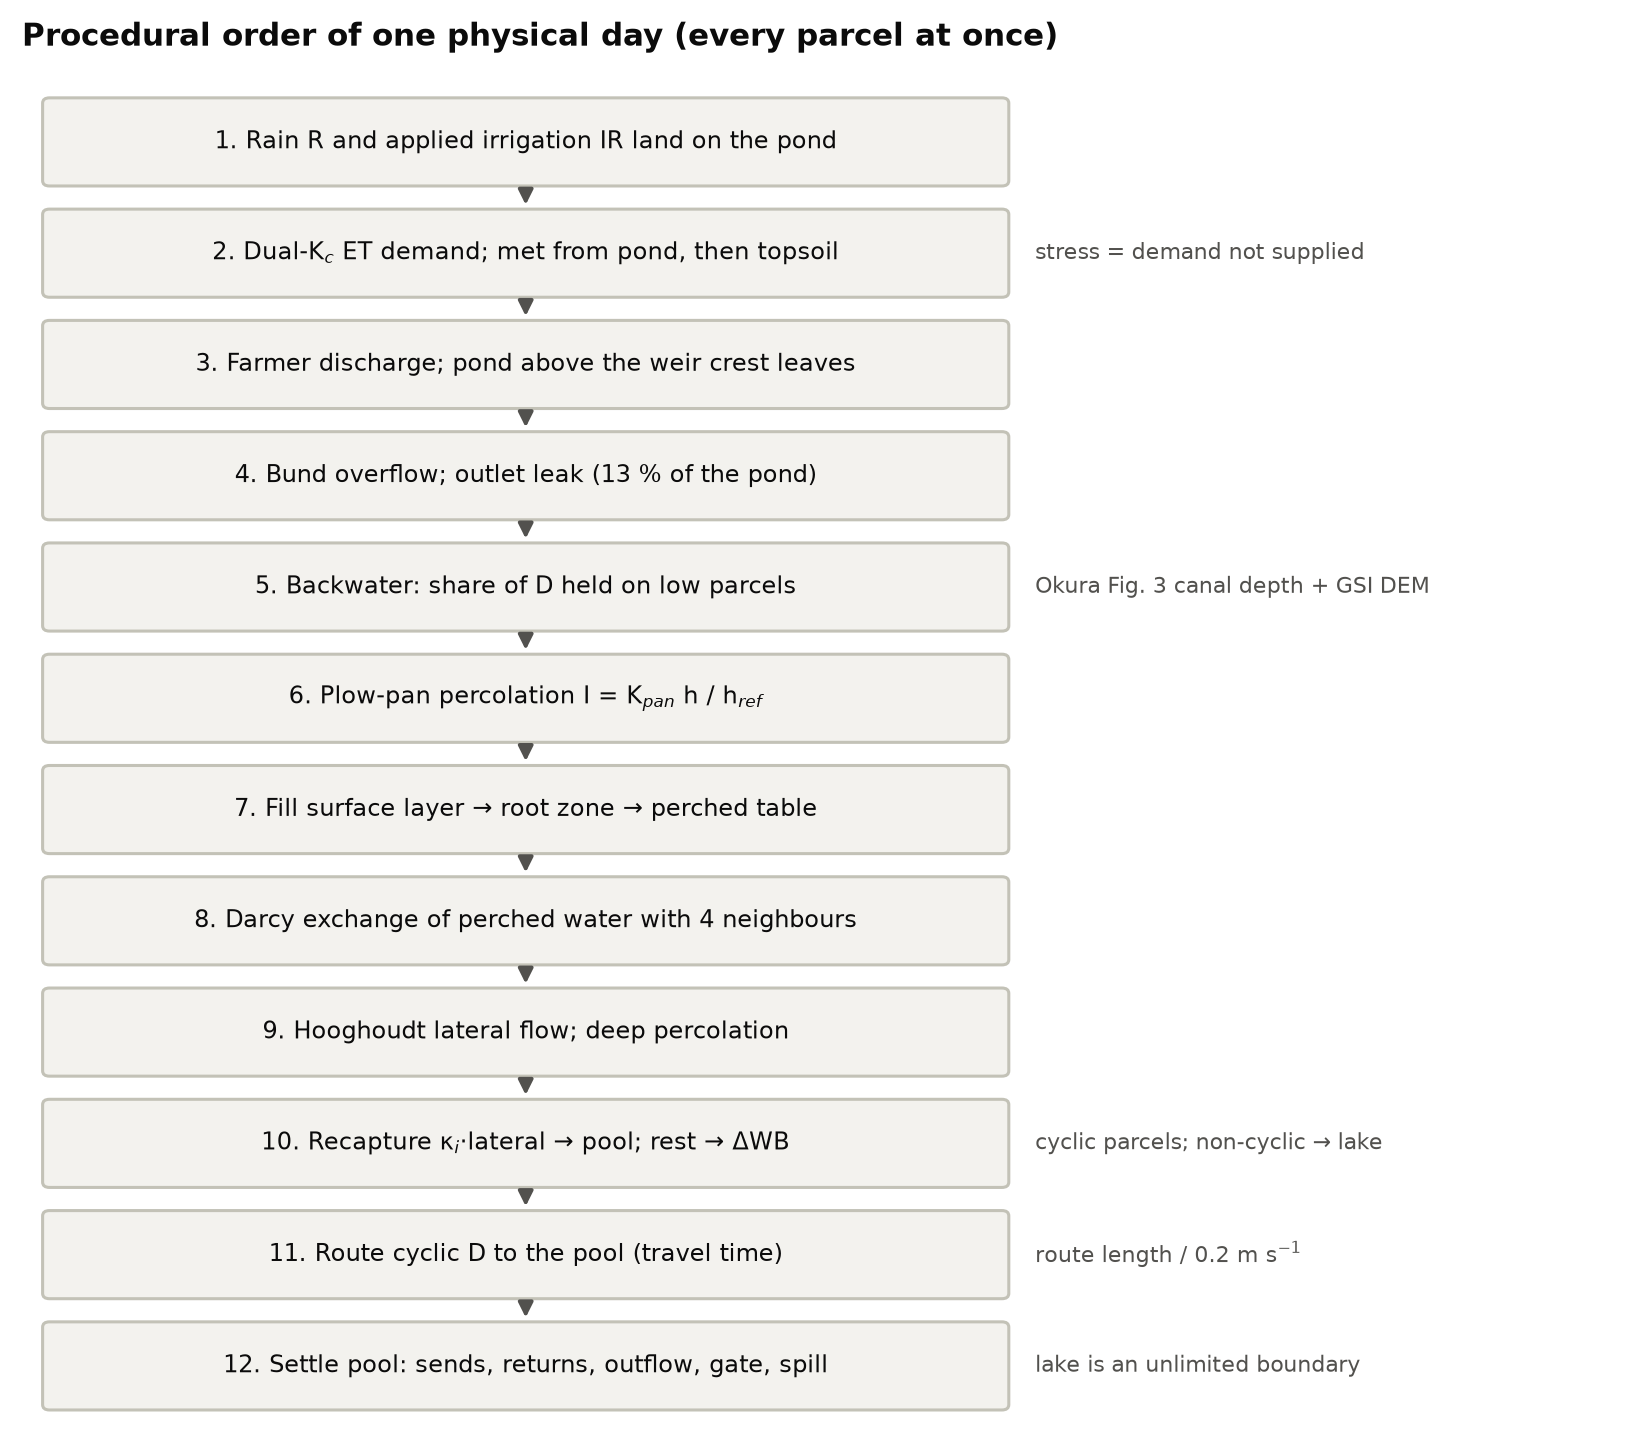
\includegraphics[width=0.82\linewidth]{fig_physics_order}
\caption{Procedural order of one day.}
\label{fig:order}
\end{figure}

\subsection{Parameters}
\begin{table}[H]
\centering\small
\begin{tabular}{L{4.6cm}L{3.0cm}L{7.6cm}}
\toprule
\textbf{Parameter} & \textbf{Value} & \textbf{Status} \\ \midrule
$K_{cb}$ bare / full canopy & 0.15 / 1.15 & FAO-56 range for rice \citep{Allen1998FAO56} \\
$K_{c,\max}$ / wetting-day cap & 1.20 / 1.29 & FAO-56; \citet{Xu2017DualKc} \\
REW / TEW & 9 / 25\,mm & FAO-56 Table 19, clay loam \\
RAW / TAW & 20 / 100\,mm & FAO-56 Table 22, rice ($p = 0.20$) \\
$K_y$ & 1.10 & \citet{Doorenbos1979} \\
$K_{pan}$, $h_{ref}$ & 9.5\,mm\,d$^{-1}$, 30\,mm & Assumed; to be calibrated \\
$K_x$, $K_y$ & 2,000\,mm\,d$^{-1}$ & Assumed; to be calibrated \\
$L$, $D_{eq}$, $\mu$ & 10\,m, 0.8\,m, 0.15 & Assumed (dense drain network) \\
Outlet leak & 13\,\% d$^{-1}$ & Assumed; to be calibrated \\
Deep percolation & 1\,mm\,d$^{-1}$ & Assumed \\
Bund height & 250\,mm & Assumed, within the 15--30\,cm of typical paddy bunds \\
Pool & $18\times68\times4$\,m & \citet{Okura2025WaterBalance}; depth assumed \\
Pump capacity & 3.304\,m$^3$\,s$^{-1}$ & MAFF Kanto \\
Drain velocity & 0.2\,m\,s$^{-1}$ & Assumed \\
Backwater band & 0.10\,m & Assumed; reference: lowest 2\,\% of cyclic land drains freely at normal canal depth \\
Recapture $\kappa_i$ & mean 0.763, 0.27--1.0 & Inferred (Section~\ref{sec:identification}) \\
\bottomrule
\end{tabular}
\caption{Parameters of the physical model and their status.}
\label{tab:params}
\end{table}

% -----------------------------------------------------------------------------
\section{Inferring the Underground Flow Ratios}
\label{sec:identification}

The physical model is run in two configurations. In the \emph{identification} configuration, described in this section, the measured block irrigation and drainage of \citet{Okura2025WaterBalance} are given as forcing, and the unknown is how the water left over after evapotranspiration is partitioned underground. In the \emph{process} configuration, used by the agent-based model (Part~\ref{part:abm}), farmers and the station decide irrigation and drainage, and the inferred shares are applied to the simulated lateral flow.

\subsection{The leftover simplex}
After irrigation, rain, drainage and evapotranspiration, the leftover $L_i$ of every parcel (Eq.~\ref{eq:lf} at parcel scale) is partitioned once into four shares that sum to one:
\begin{equation}
L_i = (K_{x,i} + K_{y,i} + K_{z,i} + K_{g,i})\,L_i, \qquad K_x + K_y + K_z + K_g = 1 .
\end{equation}
$\kappa_i = K_{x,i} + K_{y,i}$ is the \emph{recapture} share, the water that has passed the plow pan and reaches the pool the same day as part of $LFV_{pump}$; only water that has infiltrated can be recaptured. $K_z + K_g$ \emph{stays}, in the topsoil and below, and is the parcel's contribution to $\Delta WB$; it is split between the two in proportion to the evaporable and the total available water. Because the pool only sees the sum $K_x + K_y$, the split between the two axes is reported but not identified.

\subsection{Pinning the district mean}
The area-weighted mean recapture share over the cyclic parcels is fixed by the measured volumes:
\begin{equation}
\bar\kappa = \frac{LFV_{pump}}{A_N Lf_N + A_S Lf_S} = 0.738\;(2021), \qquad 0.787\;(2022).
\end{equation}

\subsection{Spatial structure}
Within that mean, parcels nearer a drain that reaches the pool recapture more. With $d_i$ the distance of parcel $i$ to the nearest such drain, a length scale $\Lambda = 400$\,m and a block intensity $\beta_{b(i)}$ that scales the North and South blocks to their measured lateral-flow depths (Okura Table~4, Fig.~6),
\begin{equation}
p_i = \beta_{b(i)}\, e^{-d_i/\Lambda}, \qquad \kappa_i = \bar\kappa\,\frac{p_i}{\langle p \rangle_A},
\end{equation}
where $\langle\cdot\rangle_A$ is the area-weighted mean over cyclic parcels. Where $\kappa_i$ would exceed one, the field is blended towards the mean so that every share remains a fraction. Measuring distance to the network of drains that reach the pool, rather than to the main canal alone, means that a parcel deep inside a block but beside a farm drain recaptures as readily as one beside the canal (Figure~\ref{fig:recapture}).

\begin{figure}[H]
\centering
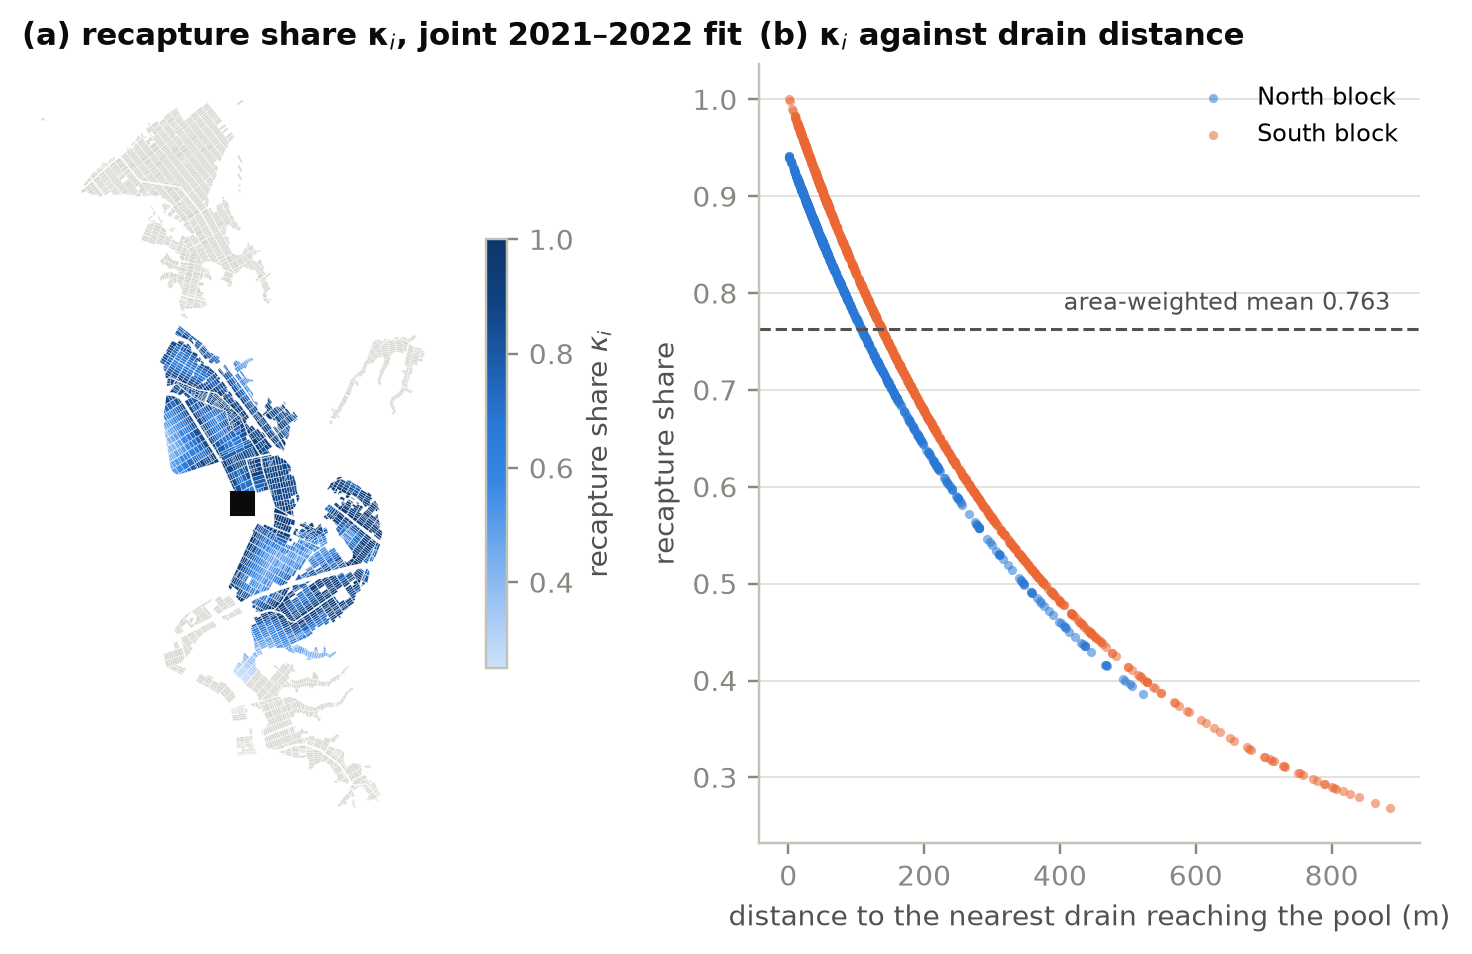
\includegraphics[width=\linewidth]{fig_recapture}
\caption{(a) The recapture share of every cyclic parcel in the joint 2021--2022 fit used by the agent-based model; non-cyclic parcels in grey. (b) The share against each parcel's distance to the nearest drain reaching the pool; the South block's higher curve is its block intensity.}
\label{fig:recapture}
\end{figure}

\subsection{Placing irrigation and drainage within a block}
\citet{Okura2025WaterBalance} measured irrigation and drainage per block, not per parcel. In the identification configuration a small neural network, trained on one year and checked on the other, distributes each day's block totals over the parcels from their pond depth, the day's ET, rain and stress, canopy cover (Sentinel-2 NDVI), block, cyclic status and distance to the canal. It covers each parcel's ET first and places the remainder, so that the block totals are met exactly while their spatial pattern follows the parcels' state.

\subsection{Holding the ratios across years}
The recapture share is fitted on one year and frozen on the other. Fitted on the wet year 2021 ($\bar\kappa = 0.738$) and applied to the dry year 2022, it lies 6.2\,\% below 2022's measured share; fitted on 2022 and applied to 2021, 6.6\,\% above. The joint fit used by the agent-based model, $\bar\kappa = 0.763$, lies within 3.1\,\% of 2022's. A share that moves by only 6--7\,\% between a season with 791\,mm of rain and one with 410\,mm behaves as a property of the district rather than of one season's weather.

\subsection{What is and is not claimed}
The contribution of this part of the model is a per-parcel map of inferred underground flow ratios, constrained by the published water balance and held across a wet and a dry year. It does not claim measured subsurface paths, a unique split between $K_x$ and $K_y$, or new knowledge of irrigation timing; lateral flow remains, as in the source study, a balance residual.

% -----------------------------------------------------------------------------
\section{Procedural Model}
\label{sec:procedural}

The physical model is the Python package \texttt{cyclic}. \texttt{cyclic.physics.advance} advances all parcels one day in the order of Figure~\ref{fig:order}; \texttt{cyclic.lateral} builds the cardinal-neighbour graph and the Darcy exchange; \texttt{cyclic.identify} computes the closed-form ratios, and \texttt{cyclic.canal} the spatial recapture field; \texttt{cyclic.infrastructure} holds the parcels, the drainage network, the elevations and the canal depths, each with its source recorded in \texttt{cyclic/bundled/SOURCES.md}. The inferred shares are frozen into a bundle (\texttt{physics\_bundle.json}) that the agent-based model loads, so that it does not rediscover them. The agent-based model's \texttt{WaterWorld} calls the same \texttt{advance} for every parcel, adds backwater, drain routing, recapture and the pool, and checks the storage identity (Eq.~\ref{eq:parcel}).

% -----------------------------------------------------------------------------
\section{Evaluation Against the Measured Water Balance}
\label{sec:evaluation}

Figure~\ref{fig:validation} compares a default season of the coupled model (the built-in farmer mix and the default station, Part~\ref{part:abm}) with the water balance measured by \citet{Okura2025WaterBalance}. Evapotranspiration is reproduced within 5--13\,\%. Irrigation is 37--46\,\% of the measured, lateral flow 24--48\,\%, and recaptured lateral flow 27--46\,\%; 2021 North drainage is within 20\,\% after backwater, but 2022 drainage is a quarter to a third of the measured.

\begin{figure}[H]
\centering
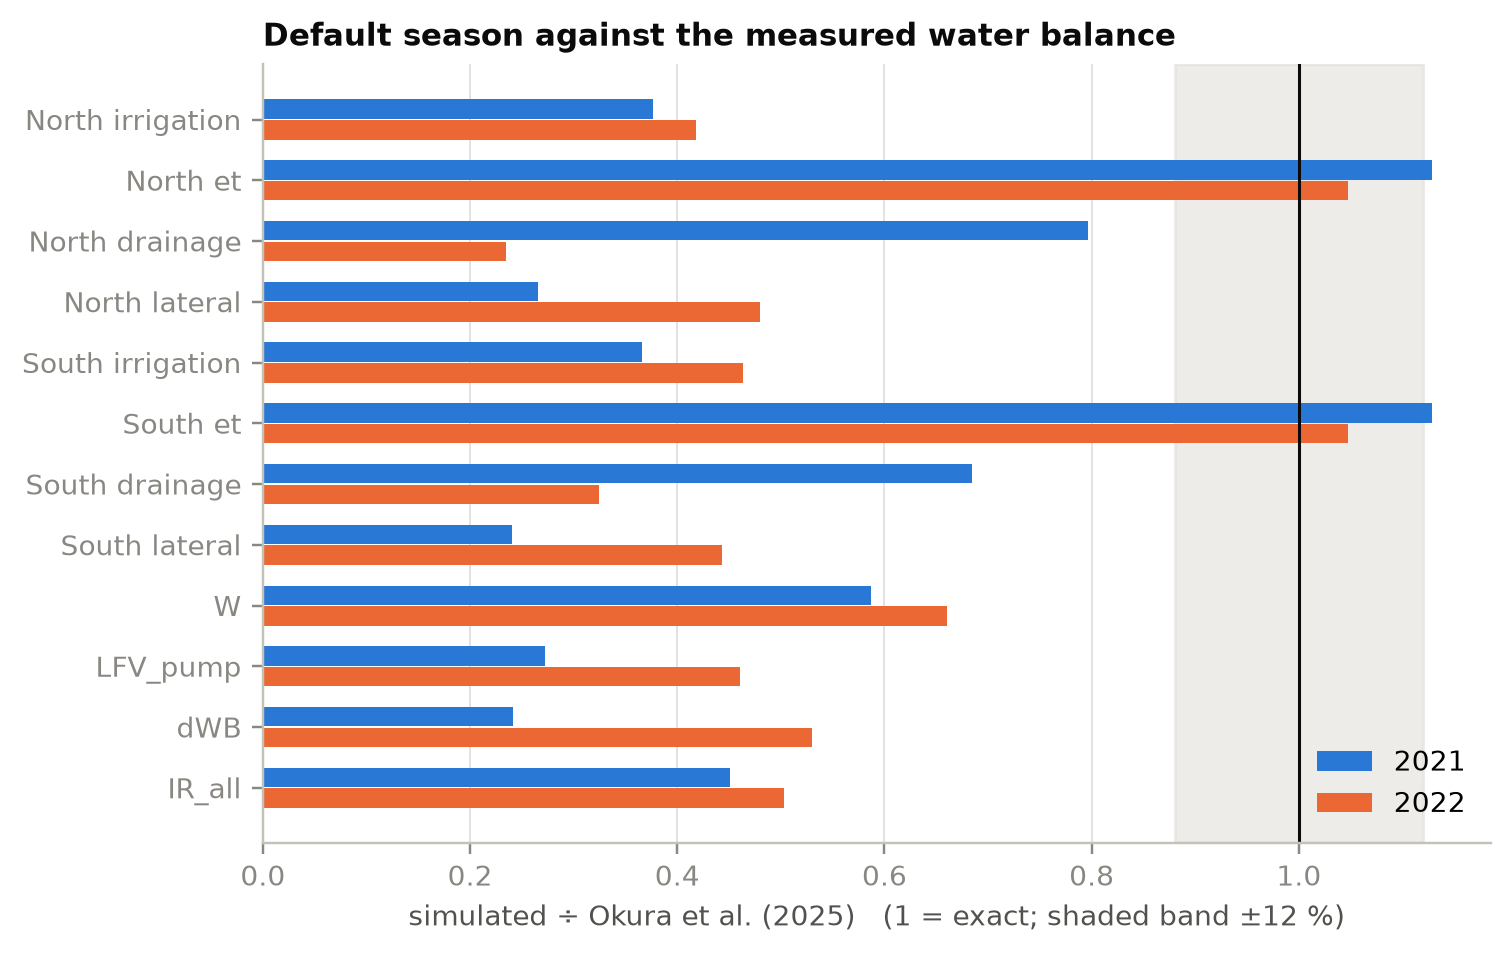
\includegraphics[width=0.85\linewidth]{fig_validation}
\caption{A default coupled season against \citet{Okura2025WaterBalance} Tables 3--6, as the ratio simulated/measured (1 = exact). Block terms in mm, station terms in volume.}
\label{fig:validation}
\end{figure}

The pattern has two causes that the evaluation separates. The irrigation deficit is a property of the decisions, not the physics: the default station sends the least water that keeps every paddy free of stress the next day, and the farmers ask for water by the rules of Part~\ref{part:abm}; the irrigators of 2021 and 2022 applied about twice as much. The lateral-flow deficit is a property of the physics: with uncalibrated soil constants and the Hooghoudt drain law, the soil sheds less water sideways than the measured residual implies (cf.\ \citealp{Ebrahimian2015Hydrus}). Calibrating $K_{pan}$, the outlet leak and the drain constants by replaying the measured irrigation and drainage is the next step, and is separate from the behavioural calibration of the agents.

% =============================================================================
\part{The Agent-Based Model (ODD+D)}
\label{part:abm}

\section{Overview}
\label{sec:overview}

\subsection{Purpose}
The agent-based model represents the farmers of the district and the LID staff at the pumping station acting on the physical model of Part~\ref{part:physical}. Its purpose is to generate behaviourally grounded irrigation demand --- what farmers ask the canal for, when and where --- under controlled weather and supply scenarios, for a downstream water-application optimiser; to quantify how individual behavioural traits and management policies shape that demand and the cyclic reuse of drainage; and to serve as the cognitive layer of a future digital twin. It is designed for researchers and for the optimiser, which can replace the station agent.

\subsection{Entities, state variables and scales}
\begin{table}[H]
\centering\small
\begin{tabular}{L{2.6cm}L{12.4cm}}
\toprule
\textbf{Entity} & \textbf{State variables} \\ \midrule
Farmer & Owned parcels; type (one of seven archetypes); twelve traits (Table~\ref{tab:traits}); learned target multiplier $m$, cooperation and drawdown tolerance; usual days off and this week's; last check day; inlet flow and weir setting left running; memory of daily outcomes; score. \\
Station & Policy and its parameters; state (\textsf{wait}, \textsf{irrigation}, \textsf{drain\_to\_lake}). \\
Parcel & The four stores of Part~\ref{part:physical}; area; block; cyclic status; owner; neighbours; recapture share; drain route; elevation; calendar shift (its owner's). \\
District & Pool; drains in transit; $\Delta WB$; day; weather; canal depth. \\
\bottomrule
\end{tabular}
\caption{Entities and state variables.}
\label{tab:entities}
\end{table}
Space is the 4,002 mapped parcels; time is daily, over the 131-day season. A farmer holds on average 50 parcels scattered across the district (about 81 farmers), drawn reproducibly from a seed; holdings can be made unequal (0.5--2 times the average).

\subsection{Process overview and scheduling}
Each day (Figure~\ref{fig:abmday}): (1) the station observes the pool, the forecast and the field deficit and decides the lake gate, the outflow and what to send to each paddy; (2) every farmer observes its own parcels and, from a snapshot of the previous day shared by all, its neighbours' strategies and scores, and decides its requests, what it applies of what was sent, its drainage and its weir boards; (3) the physical model advances (Figure~\ref{fig:order}) and the pool is settled; (4) learning farmers record the day's outcome, which they act on at their next check. Because every farmer reads the same snapshot, the order in which farmers act does not matter.

\begin{figure}[H]
\centering
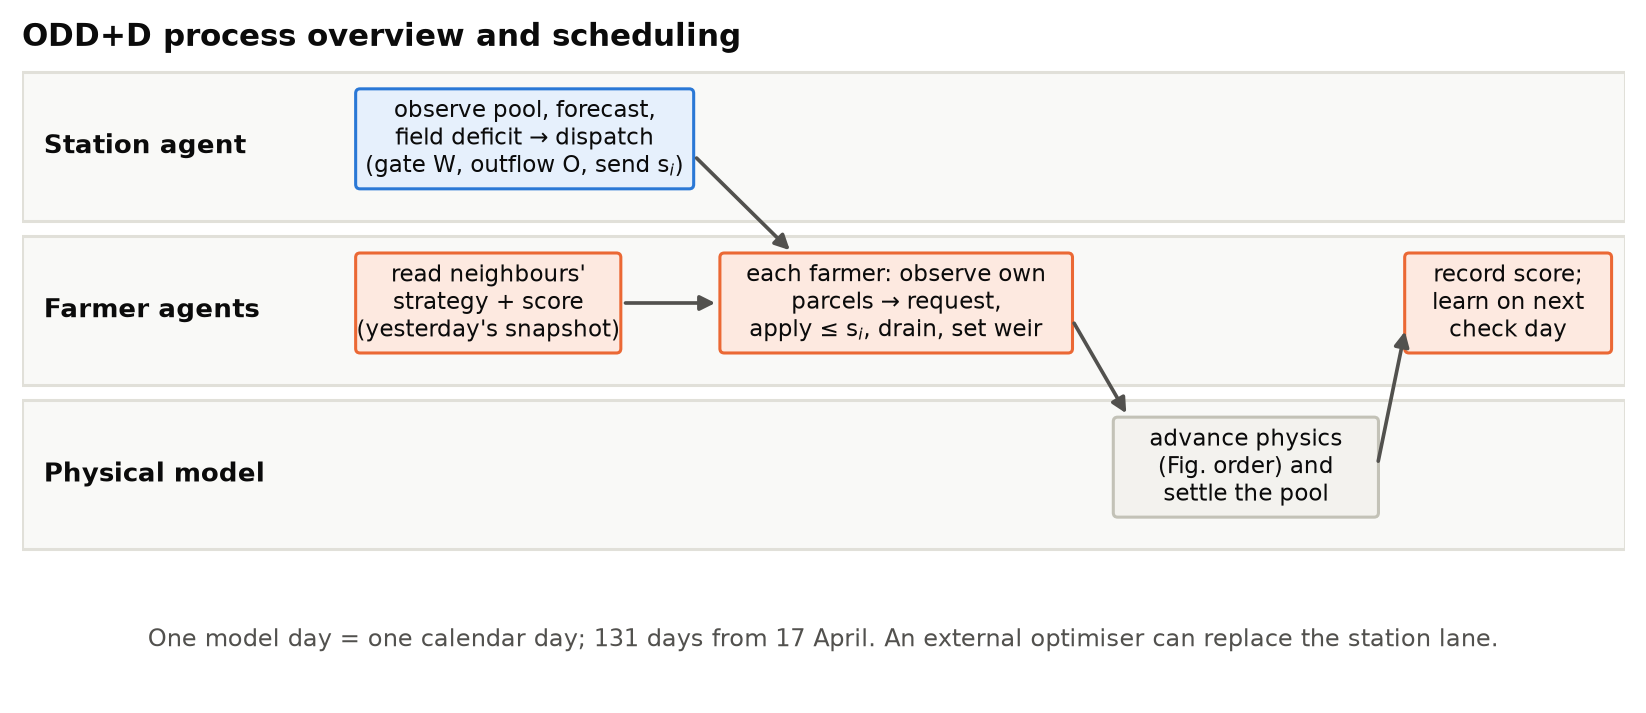
\includegraphics[width=0.95\linewidth]{fig_abm_day}
\caption{Process overview and scheduling of one model day.}
\label{fig:abmday}
\end{figure}

% -----------------------------------------------------------------------------
\section{Design Concepts}
\label{sec:design}

\subsection{Theoretical and empirical background}
Farmer behaviour follows the qualitative archetypes of the original EABSS design (Section~\ref{sec:heterogeneity}): bounded rationality, with rules of thumb for when to refill and how much, and outcome-based social learning in which farmers copy a neighbour who visibly does better \citep{Alam2022, Wens2021}. The rules encode Japanese paddy practice: fill-and-let-drop water management, the mid-season drain \citep{Itoh2011Midseason}, continuous flowing irrigation on hot days \citep{Morita2016Heat}, the no-drainage hold after herbicide application required since 2007 \citep{Phong2012Chikugo}, and farming alongside off-farm work \citep{OECD2019Japan}. The station follows receding-horizon control, the standard modern approach to canal and paddy irrigation scheduling.

\subsection{Individual decision-making}
\label{sec:decision}
The farmer's decision cycle is shown in Figure~\ref{fig:farmercycle}; the states it records, in Figure~\ref{fig:states}. A farmer's own crop calendar runs $\delta_f = \mathrm{round}(4\,\ell_f)$ days ahead of the district's, with calendar lead $\ell_f$, so its crop day is $t' = t + \delta_f$.

\begin{enumerate}
\item \textbf{Check day.} The farmer looks at its fields on its days off, and on a working day if it is at home (it is away with probability equal to its off-farm work) and its check interval $1 + 4(1 - w_f)$ days has passed ($w_f$ work ethic); never more than seven days without a look. Otherwise nothing is decided and the inlet and weir stay as left.
\item \textbf{Target.} The stage target $h^*(t')$ is 80\,mm at establishment, 60\,mm during development, 50\,mm at mid-season, 10\,mm in the mid-season drain (from crop day 70, 14 days), 30\,mm late in the season and 0 from the harvest drain at day 120; these depths are scenario assumptions. The farmer scales it by its learned multiplier and adds a risk buffer outside the drain windows, then drifts it towards its neighbours:
\begin{equation}
T = m_f h^*(t') + 8(1 - r_f), \quad T \leftarrow T + 0.3 \cdot 20 \tanh\!\left(\frac{c_f(\bar h_{nb} - T) + (1 - c_f)\,15\,b_f}{20}\right),
\end{equation}
with risk tolerance $r_f$, cooperation $c_f$, neighbour wetness bias $b_f$ and $\bar h_{nb}$ the remembered mean pond of the parcel's neighbours.
\item \textbf{Bounds.} Refill trigger $L = T - 25\,d_f$ and refill level $U = \min(T + 20\,o_f,\ \text{bund} - 20)$, with drawdown tolerance $d_f$ and refill overshoot $o_f$; in the drain windows $L = 0$ and $U = T$.
\item \textbf{Fill and let drop.} With expected daily loss $E + a_f\,\text{seep}$ ($a_f$ water accounting), $g$ days to the next check, today's counted rain $a_f R$ and the trusted forecast $\hat R = \sum_{k=1}^{\mathrm{round}(4q_f)} 0.8^k R_{t+k}$ ($q_f$ forecast reliance):
\begin{equation}
h + a_f R + \hat R - g(E + a_f\,\text{seep}) < L \ \Rightarrow\ \text{request } \max(U - \hat R, L) - h - a_f R + E + a_f\,\text{seep}.
\end{equation}
If one fill cannot last until the next check, the inlet is left trickling.
\item \textbf{Flow-through.} On hot days (ET$_0 \ge 5$\,mm) $20 k_f$\,mm is added, and while away a standing inlet $0.3 k_f$ above the expected loss ($k_f$ flow-through habit).
\item \textbf{Scarcity.} When the canal cannot meet every request, the refill is cut by $25\,\%\times c_f$.
\item \textbf{Weir.} The outlet weir crest is set at $U$.
\item \textbf{Hard rules.} Whatever a farmer type decides, it applies no more than was sent, drains no more than it holds, and keeps the water in for seven days at $\ge 30$\,mm from crop day 5 (herbicide) and, as an assumption, four days after top-dressing.
\end{enumerate}

\begin{figure}[H]
\centering
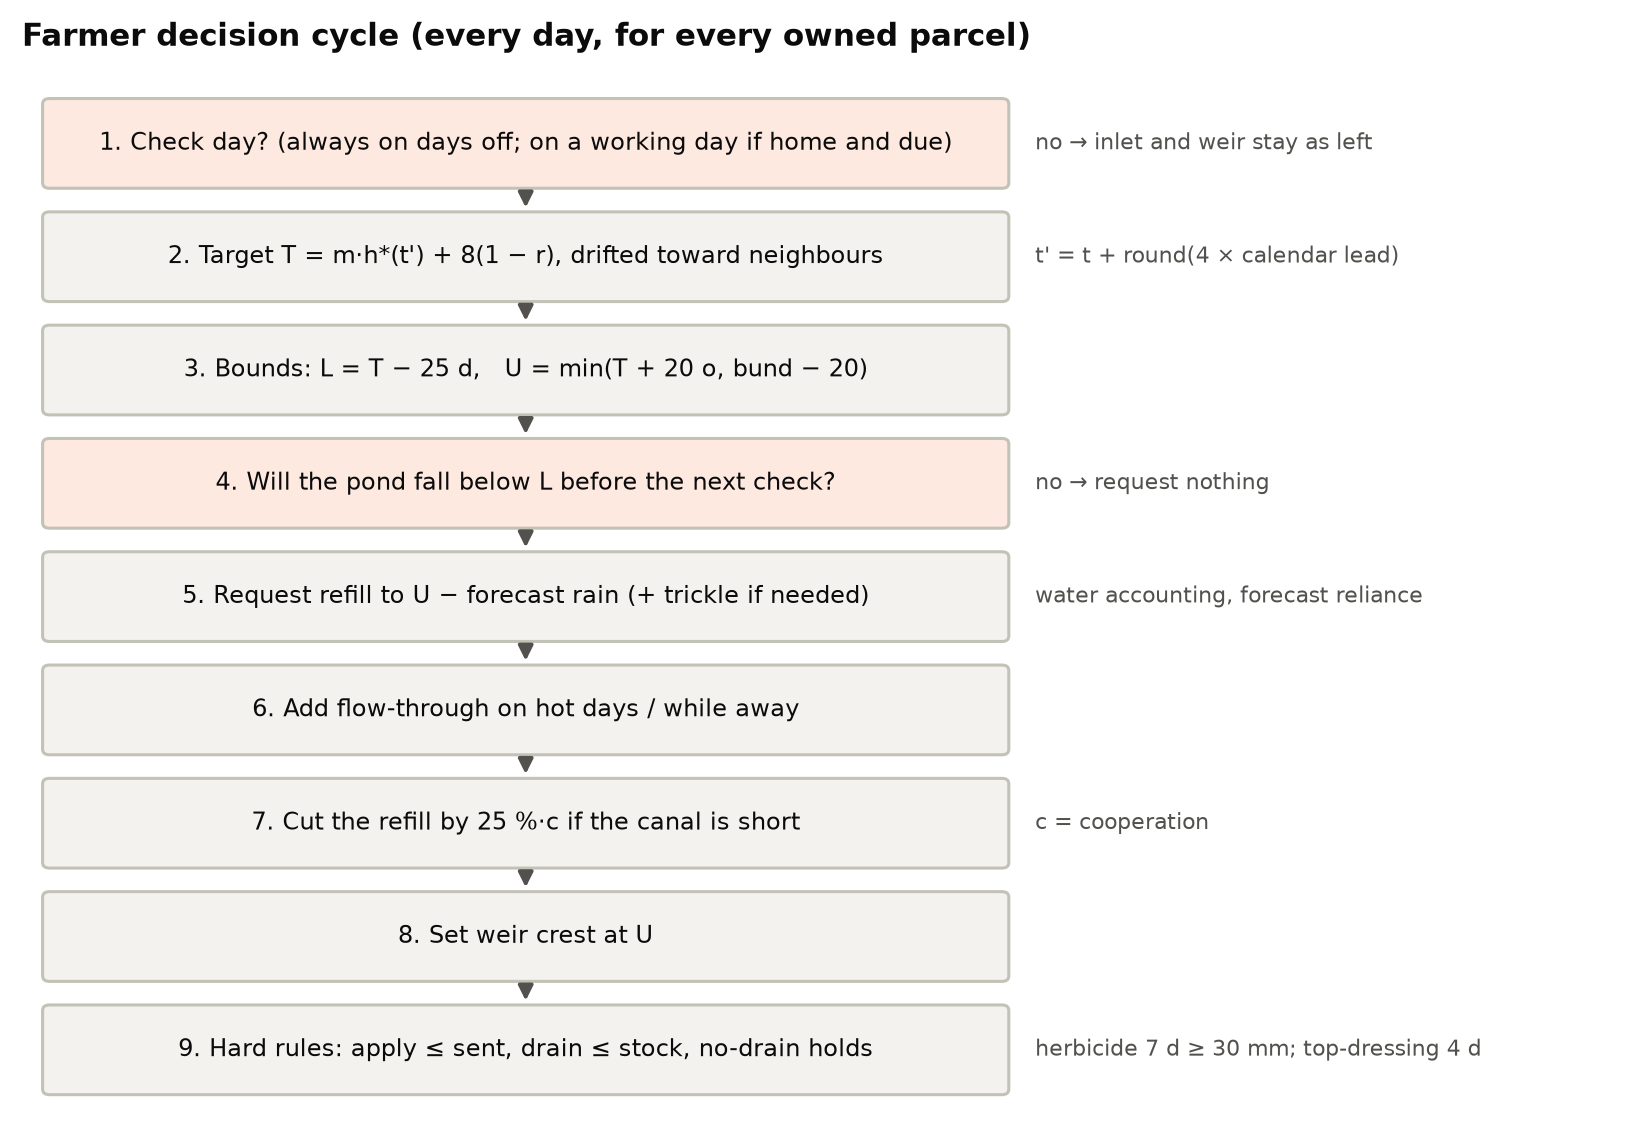
\includegraphics[width=0.92\linewidth]{fig_farmer_cycle}
\caption{Farmer decision cycle.}
\label{fig:farmercycle}
\end{figure}

\begin{figure}[H]
\centering
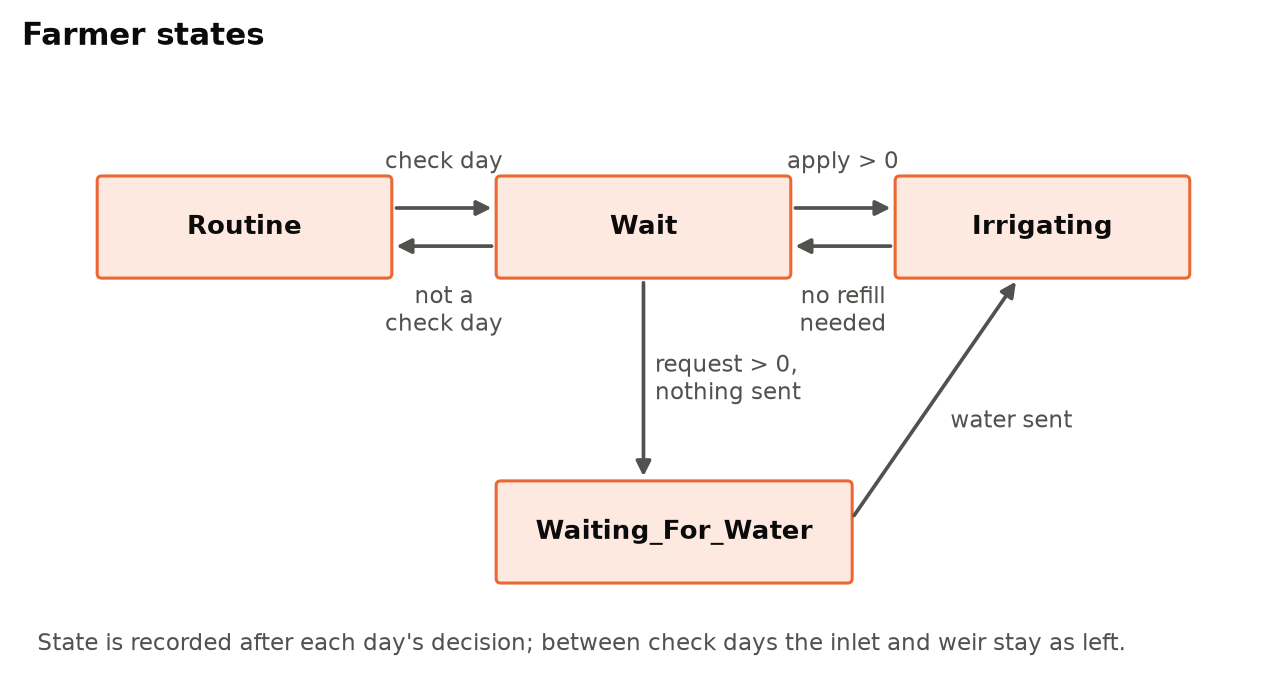
\includegraphics[width=0.62\linewidth]{fig_farmer_states}
\caption{Farmer states.}
\label{fig:states}
\end{figure}

\textbf{The station} (Figure~\ref{fig:station}) predicts every paddy's pond with a simplified version of the physical model: after a send $s$, $h_1 = \max(h_0 + R_0 + s - E_0, 0)\,\rho$ with $\rho = (1-\text{leak})(1 - K_{pan}/h_{ref})$; tomorrow is stress-free if $h_1 \ge \max(E_1 - R_1, 0) + 3$\,mm, which gives the least send
\begin{equation}
s = \frac{\max(E_1 - R_1, 0) + 3}{\rho} + E_0 - h_0 - R_0,
\end{equation}
clipped to 60\,mm\,d$^{-1}$ and the bund. Returning water (pool, same-day cyclic drainage, recaptured lateral flow) is used before lake water; the gate opens for the remaining shortfall plus 5\,\%, up to 150,000\,m$^3$\,d$^{-1}$; surplus returns are banked in cyclic paddies below target; and the pool is pumped to the lake only when $R_0 + R_1 > 40$\,mm or yesterday's spill exceeded 30,000\,m$^3$. Fixed-quota, adaptive, level-seeking and closed-gate stations implement alternative policies on the same interface.

\begin{figure}[H]
\centering
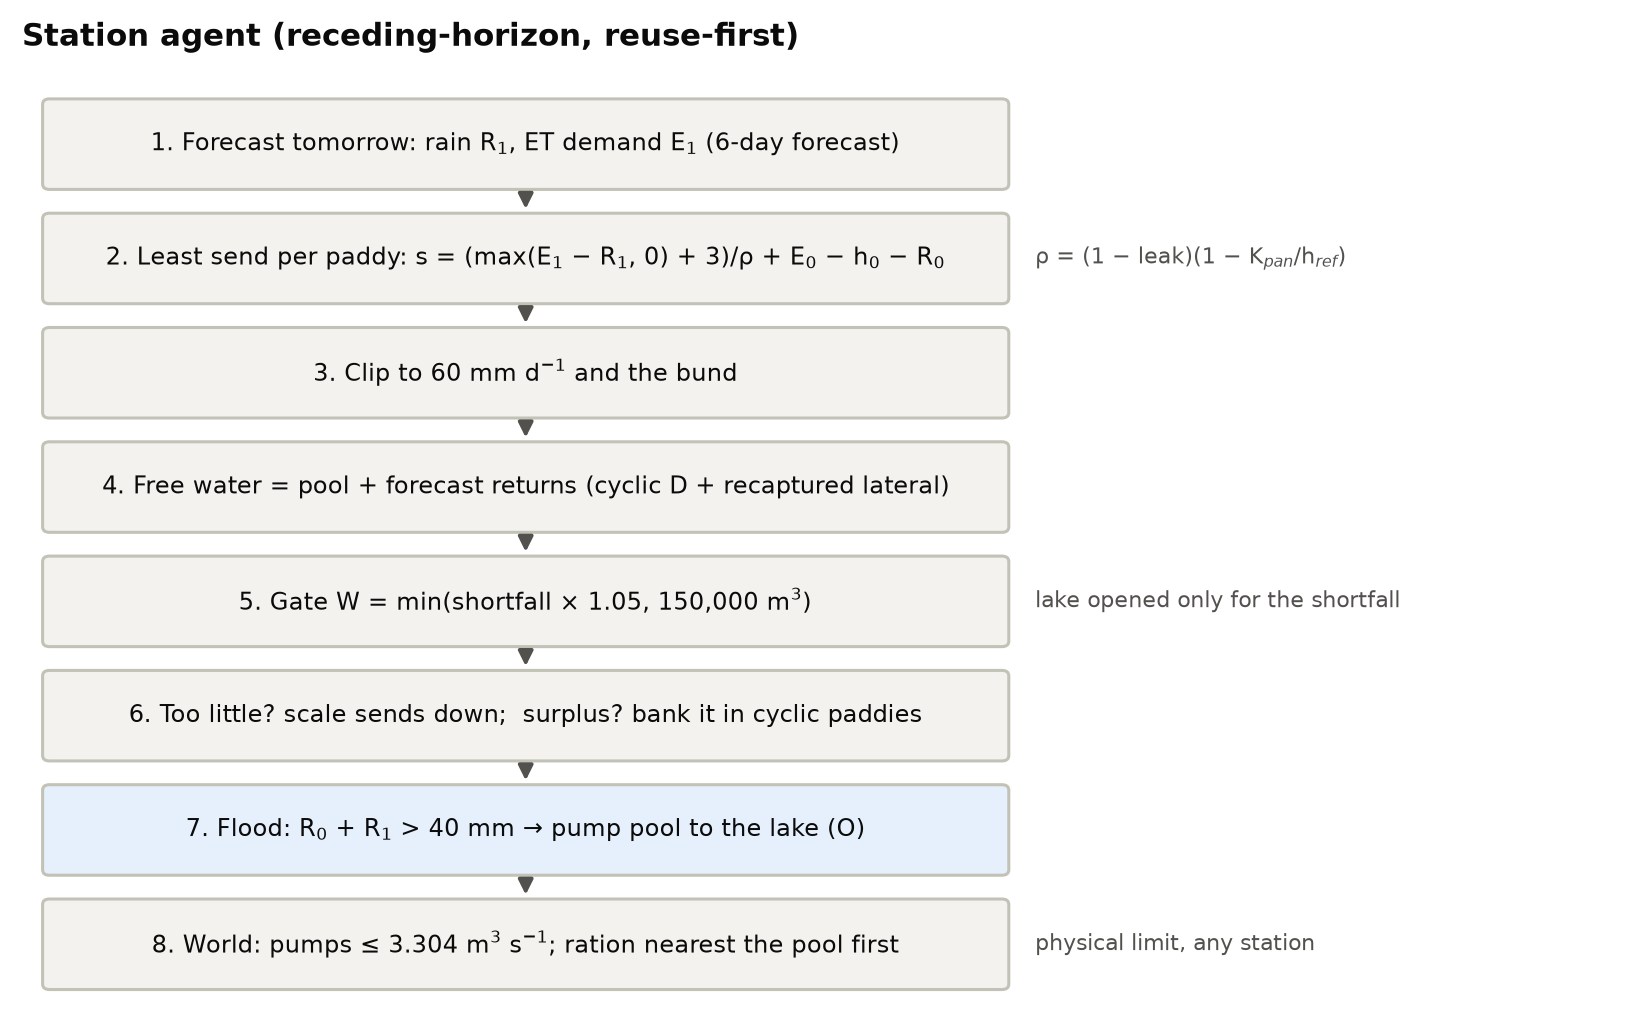
\includegraphics[width=0.92\linewidth]{fig_station}
\caption{The default station agent.}
\label{fig:station}
\end{figure}

\subsection{Learning}
On every check day a learning farmer compares its score with those of the owners of adjacent parcels. The score is an observable proxy, not profit:
\begin{equation}
S_f = \overline{K_s} - 0.15\,\overline{IR}/40 - 0.05\,\overline{D}/30 .
\end{equation}
If the best neighbour $b$ scores more than the farmer's evidence threshold above it, the farmer moves its target multiplier, cooperation and drawdown tolerance part of the way towards $b$'s: $x_f \leftarrow x_f + \lambda_f \sigma_f (x_b - x_f)$, with learning rate $\lambda_f$ and social influence $\sigma_f$. Independently, the previous day's stress and scarcity move its target, damped by experience $e_f$:
\begin{equation}
m_f \leftarrow m_f + \lambda_f\big[(1 - K_s)(1 - \tfrac{1}{2}e_f) - 0.2\,s\big], \qquad c_f \leftarrow c_f + 0.1\,\lambda_f\, s\,(1 - c_f),
\end{equation}
with $s$ the share of its request the canal could not meet; $m_f \in [0.65, 1.5]$. Learning acts within the season; $\lambda_f = 0$ gives static farmers.

\subsection{Individual sensing}
A farmer senses, on check days, the pond of each owned parcel, the water sent, yesterday's seepage loss, the crop stage on its own calendar, today's rain and a six-day rain forecast, the ponds of the four neighbours of each parcel, and its neighbours' previous-day strategy and score. It does not sense other farmers' requests or the pool. The station senses the pool, the forecast, every paddy's pond and ET demand, and the expected returns.

\subsection{Individual prediction}
Farmers predict their pond at the next check from their expected loss and the forecast rain they trust (step 4). The station predicts tomorrow's pond of every paddy and the returns it will receive.

\subsection{Interaction}
Farmers interact indirectly through the water: what one drains or seeps returns to the pool and is sent to others, and the perched table exchanges water between neighbouring parcels of different owners. They interact directly through the neighbour-relative target and social learning, both restricted to owners of adjacent parcels. The station interacts with every farmer through what it sends.

\subsection{Collectives}
Collectives are not represented as entities. A scenario can make a given share of all farmers collaborative (cooperation 0.95) and the rest uncollaborative (0.05).

\subsection{Heterogeneity}
\label{sec:heterogeneity}
Farmers differ in type, traits, holdings, days off and calendar. Each of seven archetypes fixes a mean for each of twelve traits (Tables~\ref{tab:traits} and \ref{tab:archetypes}); each farmer draws its own values around those means with a spread of 8\,\% of each trait's range. Each trait is defined by the decision rule it enters, so that its effect can be tested (Section~\ref{sec:sensitivity}).

\begin{table}[H]
\centering\small
\begin{tabular}{L{3.1cm}L{1.2cm}L{10.8cm}}
\toprule
\textbf{Trait} & \textbf{Range} & \textbf{What it does} \\ \midrule
Experience & 0--1 & Damps the rise in target after a stressed day by up to half. \\
Water accounting & 0--1 & Share of seepage loss and of today's rain counted when sizing a refill. \\
Cooperation & 0--1 & Pulls the target towards the neighbours' level; trims the refill by up to 25\,\% when the canal is short. \\
Work ethic & 0--1 & Days between checks: $1 + 4(1 - w)$. \\
Risk tolerance & 0--1 & 0 keeps an 8\,mm safety margin above the target; 1 none. \\
Neighbour wetness bias & $-1$--1 & Sits up to 15\,mm wetter ($+$) or drier ($-$) than the neighbours, as far as uncooperative. \\
Calendar lead & $-1$--1 & Crop calendar up to 4 days ahead ($+$) or behind ($-$) the district. \\
Drawdown tolerance & 0--1 & How far below target the pond may fall before a refill: up to 25\,mm. \\
Refill overshoot & 0--1 & How far above target a refill goes, and the weir crest: up to 20\,mm. \\
Off-farm work & 0--1 & Share of working days away at another job. \\
Forecast reliance & 0--1 & Days of rain forecast left room for: up to 4, trusting each later day 20\,\% less. \\
Flow-through habit & 0--1 & Inlet left running: up to 20\,mm\,d$^{-1}$ on hot days, 30\,\% above the loss while away. \\
\bottomrule
\end{tabular}
\caption{The twelve behavioural traits.}
\label{tab:traits}
\end{table}

\begin{table}[H]
\centering\scriptsize
\setlength{\tabcolsep}{3.2pt}
\begin{tabular}{lcccccccccccc}
\toprule
 & exp. & water acc. & coop. & work eth. & risk tol. & nbr.\ bias & cal.\ lead & drawdown & overshoot & off-farm & forecast & flow-thr. \\ \midrule
Maximiser & .60 & .60 & .20 & .99 & .30 & .60 & .60 & .20 & .80 & .10 & .50 & .50 \\
Survivalist & .50 & .50 & .80 & .79 & .40 & $-.50$ & $-.30$ & .70 & .20 & .70 & .30 & .10 \\
Steward & .90 & .90 & .95 & .97 & .60 & $-.30$ & .20 & .60 & .30 & .20 & .80 & .10 \\
Guardian & .95 & .70 & .50 & .92 & .10 & .50 & .40 & .10 & .70 & .20 & .40 & .30 \\
Adaptive exp. & .40 & .85 & .70 & .97 & .85 & $-.20$ & .00 & .80 & .40 & .30 & .90 & .10 \\
Passive op. & .50 & .40 & .40 & .48 & .40 & .00 & $-.70$ & .50 & .50 & .80 & .10 & .60 \\
Opportunist & .60 & .60 & .10 & .91 & .75 & .30 & .10 & .40 & .60 & .40 & .60 & .70 \\
\bottomrule
\end{tabular}
\caption{Trait means of the seven archetypes. They are scenario assumptions derived from qualitative descriptions, not values fitted to survey data. The Opportunist also takes surplus canal water beyond its request; the Adaptive Experimenter varies its requests by up to $\pm10\,\%$.}
\label{tab:archetypes}
\end{table}

\subsection{Stochasticity}
Randomness enters, all from seeds, through: parcel ownership; the assignment of archetypes to farmers; each farmer's trait draws; days off and the weeks they move; whether a part-time farmer is home on a working day; the Adaptive Experimenter's exploration; the initial pond (40--70\,mm); and, in the erratic weather scenario, day-to-day jitter of rain and ET$_0$. Trait draws use a fixed order, so pinning one trait leaves every other trait of every farmer unchanged.

\subsection{Observation}
Recorded each day for every parcel: requested, sent and applied irrigation, drainage, recaptured and retained lateral flow, pond, stress, ET; and for the district: lake withdrawal, outflow and spill, pool, returns and $\Delta WB$. Season outputs are the demand and its peak and timing, unmet demand, drainage, withdrawal, ET shortfall, relative yield, $WUE'$, $RUE$ and $LUE$ (Okura Eqs.~11--14), and the comparison with Okura Tables 3--6.

% -----------------------------------------------------------------------------
\section{Details}
\label{sec:details}

\subsection{Implementation}
The model is implemented in Python with Mesa \citep{Mesa}: \texttt{abm.model.DistrictModel} holds one Mesa agent per farmer and one for the station on \texttt{abm.world.WaterWorld} (Figure~\ref{fig:classes}). Every farmer inherits \texttt{abm.farmer.BaseFarmer}, whose decision hooks a new farmer type may override; the hard rules are enforced after any override.

\begin{figure}[H]
\centering
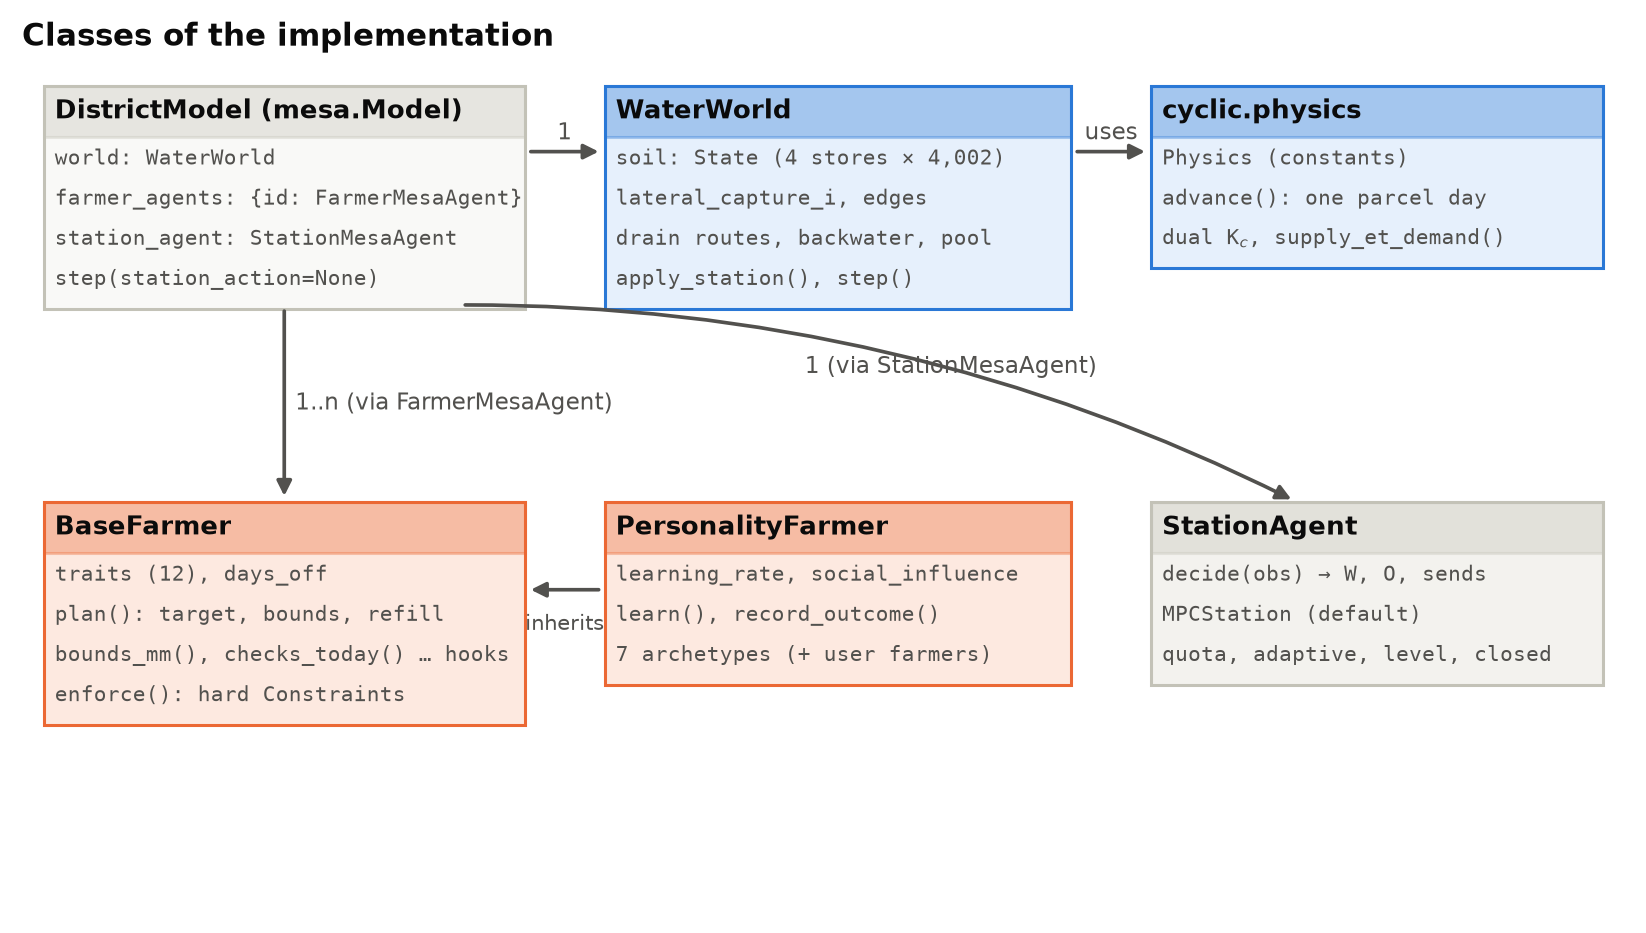
\includegraphics[width=0.95\linewidth]{fig_classes}
\caption{Classes of the implementation.}
\label{fig:classes}
\end{figure}

\subsection{Initialisation}
The district, the inferred recapture shares and the weather of the chosen year are loaded; the initial pond of every parcel is drawn between 40 and 70\,mm, the perched store set to 10\,mm and the pool filled; parcels are assigned to farmers and farmers to archetypes from the seed.

\subsection{Input data}
The forcing of Section~\ref{sec:conceptual}: daily rain and ET$_0$ (gauge-corrected, or reshaped by a weather scenario) and the main-canal depth.

\subsection{Coupling to the physical model}
\begin{table}[H]
\centering\small
\begin{tabular}{L{3.2cm}L{5.8cm}L{6.0cm}}
\toprule
 & \textbf{Reads from the physical model} & \textbf{Controls in the physical model} \\ \midrule
Farmer & Pond, seepage, ET demand on its calendar, neighbours' ponds, water sent & Applied irrigation, deliberate drainage, weir crest, crop calendar (canopy, ET) of its parcels \\
Station & Pool, ponds, ET demand, forecast returns & Lake gate $W$, outflow $O$, send to each paddy \\
\bottomrule
\end{tabular}
\caption{What the agents read from and control in the physical model.}
\label{tab:coupling}
\end{table}

\subsection{Scenarios}
Weather scenarios reshape the gauge-corrected season: drought (rain $\times0.5$, ET$_0\times1.1$, a 25-day dry spell), wet (rain $\times1.5$), heatwave (14 days at ET$_0\times1.35$ without rain), storm (150\,mm and 80\,mm on consecutive days), dry July (July rain $\times0.2$) and erratic (log-normal day-to-day jitter), in the spirit of a climate stress test \citep{Brown2012DecisionScaling}. Supply scenarios limit the pump capacity. Behavioural scenarios set the collaborative share, the learning rate, the farm structure or any trait.

% =============================================================================
\section{Verification and Sensitivity Analysis}
\label{sec:sensitivity}

Agent-based models of social-ecological systems are routinely over-parameterised relative to the data available to calibrate them \citep{TroostBerger2015}, so every behavioural trait must be shown to matter, and in the direction its rule implies. We follow the extended one-factor-at-a-time design recommended as the first step for agent-based models \citep{tenBroeke2016}: each trait is pinned for every farmer at the bottom, then at the top of its range, with everything else unchanged for the same seed, and the effect is the paired difference, so that variation between seeds cancels \citep{Lee2015Output}; three seeds were run, checked against a power analysis \citep{SeriSecchi2017}. The comparison was repeated with the pump limited to 25\,\% of its capacity, the only setting in which crops are short of water: at full capacity relative yield is 1.00 in every weather scenario, and it falls to 0.88 under the shortage. In total 168 seasons were simulated for 2022. Of 29 mechanistic expectations, 26 were met (Figure~\ref{fig:traits}).

\begin{figure}[H]
\centering
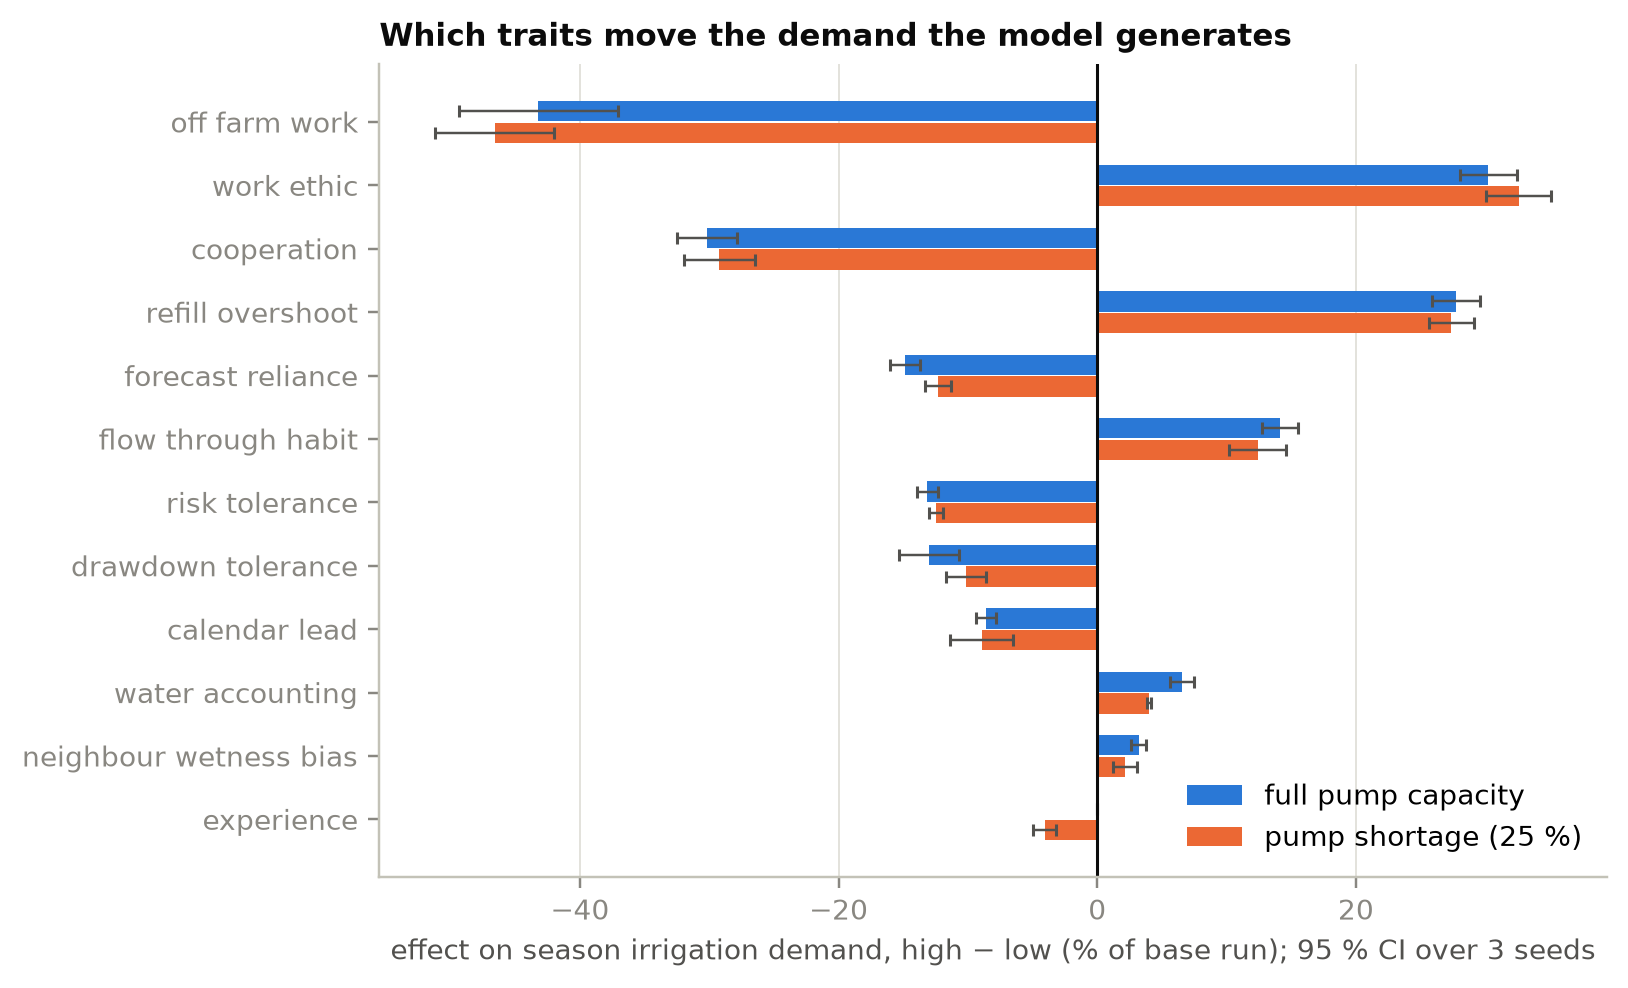
\includegraphics[width=0.88\linewidth]{fig_trait_effects}
\caption{Effect of each trait on season irrigation demand, high $-$ low, at full pump capacity and under the shortage; 95\,\% intervals over 3 seeds.}
\label{fig:traits}
\end{figure}

How often farmers are at their fields (off-farm work $-43\,\%$, work ethic $+30\,\%$) drives demand more than any preference about water depth, followed by cooperation ($-30\,\%$) and refill overshoot ($+28\,\%$). Experience has no effect at full supply and lowers demand by 4\,\% under the shortage, as its rule implies. Two expectations failed in an informative way: calendar lead delays the demand peak instead of advancing it, consistently across seeds; and under the shortage, risk tolerance lowers ponding by only 0.8\,\%, because the pond is then limited by the water sent rather than by the farmer's margin. The weather scenarios moved demand as expected (Figure~\ref{fig:scenarios}): drought $+12.6\,\%$, dry July $+3.8\,\%$, heatwave $+2.0\,\%$, wet $-8.7\,\%$.

\begin{figure}[H]
\centering
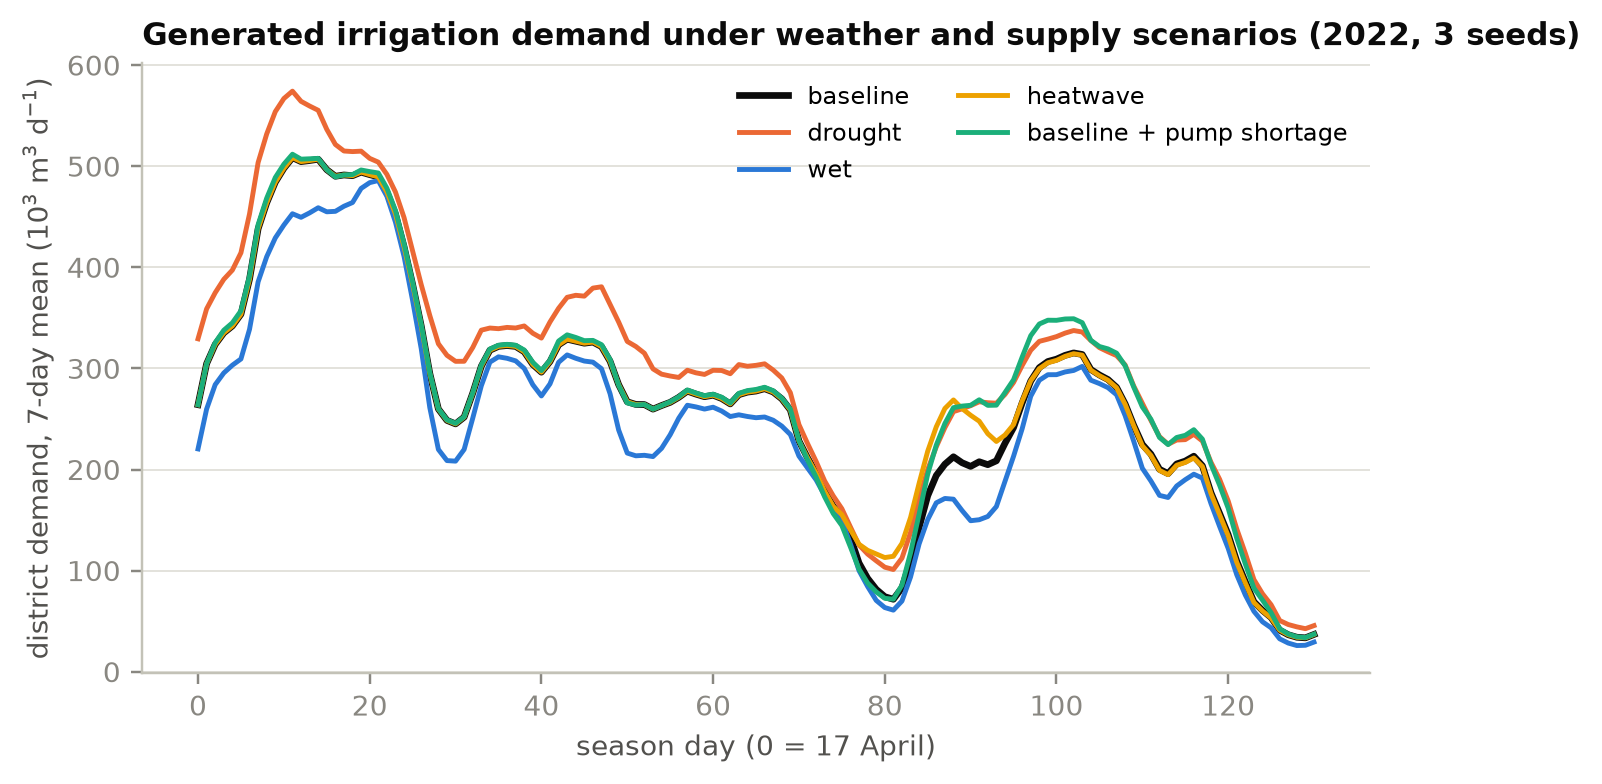
\includegraphics[width=0.92\linewidth]{fig_scenario_demand}
\caption{District irrigation demand generated under weather and supply scenarios, 7-day mean over 3 seeds, 2022.}
\label{fig:scenarios}
\end{figure}

% =============================================================================
\section{Limitations and Future Work}
\label{sec:limitations}

\textbf{Physical calibration.} The soil constants are uncalibrated, and the simulated lateral flow is a quarter to a half of the measured residual; the Hooghoudt drain law, which underestimates paddy drainage relative to the Richards equation \citep{Ebrahimian2015Hydrus}, is the first candidate for revision, alongside calibration of $K_{pan}$, the outlet leak and the conductivities by replaying the measured irrigation and drainage.

\textbf{Behavioural calibration.} The archetype means are assumptions. The sensitivity analysis shows which matter most (presence at the fields, cooperation, refill level) and therefore which a survey of Imbanuma farmers should measure first. The coupled model irrigates about half of what was measured; whether real farmers ask for more than the rules imply, or the station sends more than the least-water policy, must be resolved before the generated demand is calibrated.

\textbf{Open findings.} Calendar lead delays the demand peak. Much of what farmers request in a season is never sent, while no crop is stressed at full pump capacity; whether farmers ask for more than they need or the request counts inlets left running between checks must be resolved before the request series is used as demand for an optimiser.

\textbf{Deferred processes.} Fertiliser application and nutrient loads to the lake; volumetric water prices; pump energy cost; land abandonment; multi-season learning; and a copula-based generator of weather extremes \citep{Claassen2025}.

\textbf{Synchronisation.} Completing a digital twin requires daily irrigation and drainage series from the LID, an assimilation scheme for pond depth, and an independent actual-ET product.

\bibliographystyle{agsm}
\bibliography{bib,conceptual_model}
\end{document}
